\section{Creating the Input File: PFLOTRAN Keywords}

\setcounter{equation}{0}

The PFLOTRAN input file construction is based on keywords. Lines beginning with \# are treated as comments. Each entry to the input file must begin in the first column. Keywords {\tt SKIP} and {\tt NOSKIP} are used to skip over sections of the input file. Blank lines may occur in input file. Alternate keyword spelling is indicated in round brackets (~). Input options are indicated in square brackets [~], as well as default values. Curly brackets \{~\} indicate the result of invoking the corresponding keyword. Always refer to source code when in doubt!

Initial and boundary conditions and material properties are assigned to spatial regions using a novel {\em coupler} approach. In this approach, initial and boundary conditions (keyword CONDITION) are assigned to regions (keyword REGION) using keywords INITIAL\_CONDITION and BOUNDARY\_CONDITION. Material properties (keyword MATERIAL) are assigned to regions using the keyword STRATIGRAPHY.

\begin{longtable}{ll}%[h]%\centering
%\caption{PFLOTRAN Keywords}\label{flkeywd}

%\vspace{4mm}

%\begin{tabular}{lll}
\toprule[1.5pt]
\multicolumn{1}{c}{\hypertarget{target_key}{\bf Keyword}} & \multicolumn{1}{c}{\bf Description}\\
\midrule[1pt]
\hyperlink{target_bcon}{\bf BOUNDARY\_CONDITION} & \\
%\hyperlink{target_brk}{\bf BREAKTHROUGH} & \\
\hyperlink{target_brine}{\bf BRINE} & \\
\hyperlink{target_charcrv}{\bf CHARCTERISTIC\_CURVES} & \\
\hyperlink{target_ckpt}{\bf CHECKPOINT} & \\
\hyperlink{target_chem}{\bf CHEMISTRY} & \\
\hyperlink{target_stat}{\bf COMPUTE\_STATISTICS} & \\
\hyperlink{target_co2dat}{\bf CO2\_DATABASE} & \\
\hyperlink{target_constraint}{\bf CONSTRAINT} & transport (optional)\\
\hyperlink{target_datset}{\bf DATASET} & \\
\hyperlink{target_dbase}{\bf DBASE\_DATASET} & \\
\hyperlink{target_dbg}{\bf DEBUG} & \\
\hyperlink{target_eos}{\bf EOS} & \\
\hyperlink{target_flow_cond}{\bf FLOW\_CONDITION} & \\
\hyperlink{target_fluid_property}{\bf FLUID\_PROPERTY} & \\
\hyperlink{target_geomech}{\bf GEOMECHANICS} & \\
\hyperlink{target_geomech_grid}{\bf GEOMECHANICS\_GRID} & \\
\hyperlink{target_geomech_output}{\bf GEOMECHANICS\_OUTPUT} & \\
\hyperlink{target_geomech_material_prop}{\bf GEOMECHANICS\_MATERIAL\_PROPERTY} & \\
\hyperlink{target_geomech_region}{\bf GEOMECHANICS\_REGION} & \\
\hyperlink{target_geomech_condition}{\bf GEOMECHANICS\_CONDITION} & \\
\hyperlink{target_geomech_bc}{\bf GEOMECHANICS\_BOUNDARY\_CONDITION} & \\
\hyperlink{target_geomech_strata}{\bf GEOMECHANICS\_STRATA} & \\
\hyperlink{target_grid}{\bf GRID} & (required)\\
\hyperlink{target_init}{\bf INITIAL\_CONDITION} & \\
\hyperlink{target_int_flux}{\bf INTEGRAL\_FLUX} & \\
\hyperlink{target_linsolv}{\bf LINEAR\_SOLVER} & \\
\hyperlink{target_mat}{\bf MATERIAL\_PROPERTY} & \\
\hyperlink{target_mode}{\bf MODE} & \\
\hyperlink{target_mc}{\bf MULTIPLE\_CONTINUUM} & \\
\hyperlink{target_newt}{\bf NEWTON\_SOLVER} & \\
\hyperlink{target_nonuniform_vel}{\bf NONUNIFORM\_VELOCITY} & \\ 
\hyperlink{target_numjac_flow}{\bf NUMERICAL\_JACOBIAN\_FLOW} & \\
\hyperlink{target_numjac_rxn}{\bf NUMERICAL\_JACOBIAN\_RXN} & \\
\hyperlink{target_numjac_multi}{\bf NUMERICAL\_JACOBIAN\_MULTI\_COUPLE} & \\
\hyperlink{target_observation}{\bf OBSERVATION} & \\
\hyperlink{target_orig}{\bf ORIG, ORIGIN} & \\
\hyperlink{target_output}{\bf OUTPUT} & \\
\hyperlink{target_overwrite}{\bf OVERWRITE\_RESTART\_TRANSPORT} & \\
\hyperlink{target_proc}{\bf PROC} & (optional)\\
\hyperlink{target_region}{\bf REGION} & \\
\hyperlink{target_restart}{\bf RESTART} & \\
\hyperlink{target_sat}{\bf SATURATION\_FUNCTION} & \\
\hyperlink{target_src}{\bf SOURCE\_SINK} & \\
\hyperlink{target_strata}{\bf STRATIGRAPHY (STRATA)} & \\
\hyperlink{target_time}{\bf TIME} & \\
\hyperlink{target_timestep}{\bf TIMESTEPPER} & \\
\hyperlink{target_trans_cond}{\bf TRANSPORT\_CONDITION} & \\
\hyperlink{target_unifvel}{\bf UNIFORM\_VELOCITY} & \\
\hyperlink{target_touch}{\bf USE\_TOUCH\_OPTIONS} & \\
\hyperlink{target_veldata}{\bf VELOCITY\_DATASET} & (optional) \\
\hyperlink{target_wallclk}{\bf WALLCLOCK\_STOP} & \\
\bottomrule[1.5pt]
%\end{tabular}
\end{longtable}


\subsection{Conventions and Notation} 

Keywords are in boldface with optional modifying keywords in square brackets [\ldots], and user entries in typewriter font.
Unless otherwise specified, units in the input file are assumed to be as listed in Table~\ref{tunits}.

\begin{table}[h]\centering
\caption{Units}\label{tunits}

\vspace{3mm}

%\rowcolors{row}{odd-row cyan}{even-row green}
%\rowcolors[]{1}{red!20}{red!10}
%\rowcolors[]{1}{blue!20}{blue!10}
\rowcolors[]{1}{teal!20}{teal!10}
%\rowcolors{1}{}{lightgray}
%\rowcolors{1}{}{teal}
\begin{tabular}{ll}
\toprule[2pt]
%\hline
%Quantity & \multicolumn{1}{c}{Units}\\
Quantity & \multicolumn{1}{c}{Units}\\
\midrule[1pt]
%\hline
Pressure: & Pascal [Pa] (absolute)\\
%\rowcolor[rgb]{0.5}
Temperature: & Celcius [C]\\
Distance: & meter [m]\\
Volume: & meter$^3$ [m$^3$]\\
Time: & second [s]\\
Velocity: & meter/second [m/s]\\
Concentration: & molarity [M] or molality [m] (see MOLAL keyword)\\
Enthalpy: & kiloJoule/mole [kJ/mol]\\
Mass: & kilogram [kg]\\
Rate: & kilogram/second [kg/s] or cubic meter/second [m$^3$/s]\\
Surface Site Density: & mole/meter$^{3}$ [mol/m$^{3}$]\\
\bottomrule[1.5pt]
%\hline
\end{tabular}
\end{table}

\begin{comment}
\begin{verbatim}
\protect\hypertarget{target_XXX}{}
\subsection{Keyword: XXX}
{\noindent\bf Description:}
{\noindent\bf Input:}
\begin{deflist}{0000000000}
\item[]
\end{deflist}
{\noindent\bf Explanation:}
\begin{description}
\item[Keyword XXX]
\end{description}
{\noindent\bf Examples:}
\end{verbatim}
\end{comment}

\clearpage

\subsection{Example Input File}\label{exinput}

\hypertarget{target_input_file}{}

\footnotesize
\#Description: 3D infiltration problem with calcite dissolution
(\# denotes a comment line)\\

\noindent
\# == debugging ================================================================\\
\#\hyperlink{target_dbg}{\bf DEBUG}\\
%\hypertarget{target_key}{\bf DEBUG}\\
\#  MATVIEW\_JACOBIAN\\
\#  VECVIEW\_RESIDUAL\\
\#  VECVIEW\_SOLUTION\\
\#/

\noindent
\# == mode =====================================================================\\
\hyperlink{target_mode}{\bf MODE} RICHARDS

\noindent
\# == chemistry ================================================================\\
\hyperlink{target_chem}{\bf CHEMISTRY}\\
OPERATOR\_SPLIT\\
PRIMARY\_SPECIES\\
  Ca++\\
  H+\\
  CO2(aq)\\
  Tracer\\
/\\
SECONDARY\_SPECIES\\
  OH$-$\\
  HCO3$-$\\
  CO3$-$$-$\\
  CaHCO3+\\
  CaCO3(aq)\\
/\\
GAS\_SPECIES\\
  CO2(g)\\
/\\
MINERALS\\
  Calcite\\
/\\
\#\\
MINERAL\_KINETICS\\
Calcite\\
RATE\_CONSTANT 1.e-8 ! [mol/m$^2$/s]\\
/\\
/\\
\#\\
DATABASE /Users/lichtner/flotran/database/hanford.dat\\
LOG\_FORMULATION\\
ACTIVITY\_COEFFICIENTS !NEWTON\_ITERATION\\
MOLAL\\
OUTPUT\\
All\\
/\\
/

\noindent
\# == reference variables ======================================================\\
REFERENCE\_POROSITY 0.25d0\\

\noindent
\# == time stepping ============================================================\\
\hyperlink{target_timestep}{\bf TIMESTEPPER}\\
TS\_ACCELERATION 8\\
MAX\_STEPS 100000\\
/

\noindent
\# == discretization ===========================================================\\
\hyperlink{target_grid}{\bf GRID}\\
%\#TYPE amr ! amr grid\\
TYPE structured\\
NXYZ 6 6 6\\
BOUNDS\\
0.d0 0.d0 0.d0\\
1.d0 1.d0 1.d0\\
/\\
\#DXYZ\\
\#1.\\
\#1.\\
\#1.\\
\#/\\
/

\noindent
\# == flow solvers =============================================================\\
\hyperlink{target_newt}{\bf NEWTON\_SOLVER} FLOW\\
PRECONDITIONER\_MATRIX\_TYPE AIJ\\
RTOL 1.d-8\\
ATOL 1.d-8\\
STOL 1.d-30\\
ITOL\_UPDATE 1.d0\\
\#NO\_INFINITY\_NORM\\
\#NO\_PRINT\_CONVERGENCE\\
\#PRINT\_DETAILED\_CONVERGENCE\\
/

\noindent
\hyperlink{target_linsolv}{\bf LINEAR\_SOLVER} FLOW\\
\#KSP\_TYPE PREONLY\\
\#PC\_TYPE LU\\
\#KSP\_TYPE FGMRES !samrai\\
\#PC\_TYPE SHELL !samrai\\
/

\noindent
\# == transport solvers ========================================================\\
\hyperlink{target_newt}{\bf NEWTON\_SOLVER} TRANSPORT\\
PRECONDITIONER\_MATRIX\_TYPE AIJ\\
RTOL 1.d-12\\
ATOL 1.d-12\\
STOL 1.d-30\\
\#NO\_INFINITY\_NORM\\
\#NO\_PRINT\_CONVERGENCE\\
\#PRINT\_DETAILED\_CONVERGENCE\\
/

\noindent
\hyperlink{target_linsolv}{\bf LINEAR\_SOLVER} TRANSPORT\\
\#PC\_TYPE LU\\
\#KSP\_TYPE PREONLY\\
\#KSP\_TYPE FGMRES ! samrai\\
\#PC\_TYPE SHELL !samrai\\
/

\noindent
\# == fluid properties =========================================================\\
\hyperlink{target_fluid_property}{\bf FLUID\_PROPERTY}\\
DIFFUSION\_COEFFICIENT 1.d-9\\
/

\noindent
\#\hyperlink{target_unifvel}{\bf UNIFORM\_VELOCITY} 3.84259d-6 0.d0 0.d0  ! 1.38333 cm/h

\noindent
\# == material properties ======================================================\\
\hyperlink{target_mat}{\bf MATERIAL\_PROPERTY} HD\\
ID 1\\
SATURATION\_FUNCTION HD\\
POROSITY 0.262\\
TORTUOSITY 1.0\\
PERMEABILITY\\
PERM\_ISO 5.43d-13\\
/\\
/

\noindent
\# == saturation / permeability functions ======================================\\
\hyperlink{target_sat}{\bf SATURATION\_FUNCTION} HD\\
SATURATION\_FUNCTION\_TYPE VAN\_GENUCHTEN\\
RESIDUAL\_SATURATION 0.115\\
LAMBDA 0.286\\
ALPHA 1.9401d-4\\
/

\noindent
\# == output ===================================================================\\
\hyperlink{target_output}{\bf OUTPUT}\\
\#PERIODIC TIMESTEP 1\\
PERIODIC TIME 0.1 y\\
FORMAT HDF5\\
FORMAT TECPLOT BLOCK\\
VELOCITIES\\
/

\noindent
\# == times ====================================================================\\
\hyperlink{target_time}{\bf TIME}\\
FINAL\_TIME 1.d0 y\\
INITIAL\ 1.e-6 y\\
MAXIMUM\_TIMESTEP\_SIZE 1.e-2 y\\
/

\noindent
\# == regions ==================================================================\\
\hyperlink{target_region}{\bf REGION} all\\
COORDINATES\\
0.d0 0.d0 0.d0\\
6.d0 6.d0 6.d0\\
/\\
/

\noindent
\hyperlink{target_region}{\bf REGION} Top\\
FACE TOP\\
COORDINATES\\
0.d0 0.d0 6.d0\\
6.d0 6.d0 6.d0\\
/\\
/

\noindent
\hyperlink{target_region}{\bf REGION} Inlet\\
FACE TOP\\
COORDINATES\\
2.d0 2.d0 6.d0\\
4.d0 4.d0 6.d0\\
/\\
\#BLOCK 3 4 3 4 6 6\\
/

\noindent
\hyperlink{target_region}{\bf REGION} Bottom\\
FACE BOTTOM\\
COORDINATES\\
0.d0 0.d0 0.d0\\
6.d0 6.d0 0.d0\\
/\\
/

\noindent
\# == flow conditions ==========================================================\\
\hyperlink{target_flow_cond}{\bf FLOW\_CONDITION} Inlet\\
TYPE\\
FLUX neumann\\
/\\
FLUX 0.317098d-6 ! 10 m/y\\
/

\noindent
\hyperlink{target_flow_cond}{\bf FLOW\_CONDITION} Initial\\
TYPE\\
PRESSURE hydrostatic\\
/\\
DATUM 0.d0 0.d0 6.d0\\
PRESSURE 101325.d0\\
/

\noindent
\# == transport conditions =====================================================\\
\hyperlink{target_trans_cond}{\bf TRANSPORT\_CONDITION} Inlet\\
TYPE dirichlet\\
CONSTRAINT\_LIST\\
0.d0 Inlet\\
/\\
/

\noindent
\hyperlink{target_trans_cond}{\bf TRANSPORT\_CONDITION} Initial\\
TYPE dirichlet\\
CONSTRAINT\_LIST\\
0.d0 Initial\\
/\\
/

\noindent
\hyperlink{target_trans_cond}{\bf TRANSPORT\_CONDITION} Outlet\\
TYPE zero\_gradient\\
CONSTRAINT\_LIST\\
0.d0 Initial\\
/\\
/

\noindent
\# == couplers =================================================================\\
\hyperlink{target_bcon}{\bf BOUNDARY\_CONDITION} Inlet\\
\hyperlink{target_flow_cond}{\bf FLOW\_CONDITION} Inlet\\
\hyperlink{target_trans_cond}{\bf TRANSPORT\_CONDITION} Inlet\\
\hyperlink{target_region}{\bf REGION} Inlet\\
/

\noindent
\hyperlink{target_bcon}{\bf BOUNDARY\_CONDITION} Outlet\\
\hyperlink{target_flow_cond}{\bf FLOW\_CONDITION} Initial\\
\hyperlink{target_trans_cond}{\bf TRANSPORT\_CONDITION} Outlet\\
\hyperlink{target_region}{\bf REGION} Bottom\\
/

\noindent
\hyperlink{target_init}{\bf INITIAL\_CONDITION} Initial\\
\hyperlink{target_flow_cond}{\bf FLOW\_CONDITION} Initial\\
\hyperlink{target_trans_cond}{\bf TRANSPORT\_CONDITION} Initial\\
\hyperlink{target_region}{\bf REGION} all\\
/

\noindent
\# == stratigraphy =============================================================\\
\hyperlink{target_strata}{\bf STRATA}\\
MATERIAL HD\\
REGION all\\
/

\noindent
\# == transport constraints ======================================================\\
\hyperlink{target_constraint}{\bf CONSTRAINT} Initial\\
CONCENTRATIONS\\
Ca++    1.d-4   M  Calcite\\
H+      8.d0   pH\\
CO2(aq) 1.d-2   G  CO2(g)\\
Tracer  1.d-8   T\\
/\\
MINERALS ! vol. frac.  area\\
Calcite      0.75      1.d2\\
/\\
/

\noindent
\hyperlink{target_constraint}{\bf CONSTRAINT} Inlet\\
CONCENTRATIONS\\
Ca++    1.d-6   T\\
H+      3.d0   pH\\
CO2(aq) 1.d-3   G  CO2(g)\\
Tracer  1.d-0   T\\
/\\
/
\normalsize

\newpage
\protect\hypertarget{target_bcon}{}

\subsection{Keyword: BOUNDARY\_CONDITION}
{\noindent\bf Description:}
The BOUNDARY\_CONDITION keyword couples conditions specified under the FLOW\_\-CONDITION and/or TRANSPORT\_CONDITION keywords to a REGION in the problem domain.  The use of this keyword enables the use/reuse of flow and transport conditions and regions within multiple boundary and initial conditions and source/sinks in the input deck.

{\noindent\bf Input:}

\begin{deflist}{000}
\item[BOUNDARY\_CONDITION] {\tt boundary\_condition\_name}
\begin{deflist}{000}
\item[FLOW\_CONDITION] {\tt flow\_condition\_name}
\item[TRANSPORT\_CONDITION] {\tt transport\_condition\_name}
\item[REGION] {\tt region\_name}
\end{deflist}
\item[\keyend]
\end{deflist}

{\noindent\bf Explanation:}

\begin{center}
\begin{tabularx}{\linewidth}{lX}
\toprule[1.5pt]
\bf Keyword & \bf Description\\
\midrule
\bf BOUNDARY\_CONDITION & Defines the beginning of a boundary condition entry and the name of the boundary condition.\\
\midrule
\bf FLOW\_CONDITION & Defines the name of the flow condition to be linked to this boundary condition.\\
\midrule
\bf TRANSPORT\_CONDITION & Defines the name of the transport condition to be linked to this boundary condition.\\
\midrule
\bf REGION & Defines the name of the region to which the conditions are linked.\\
\midrule
\bf END & Terminates the boundary condition entry.\\
%\midrule\midrule
\bottomrule[1.5pt]
\end{tabularx}
\end{center}

\bigskip

\newpage
\begin{mdframed}

{\noindent\bf Examples:}

\begin{verbatim}
BOUNDARY_CONDITION river
  FLOW_CONDITION river_stage
  TRANSPORT_CONDITION river_chemistry
  REGION river_bank
END

BOUNDARY_CONDITION recharge
  FLOW_CONDITION infiltration_flux
  TRANSPORT_CONDITION infiltration_chemistry
  REGION ground_surface
END
\end{verbatim}

\end{mdframed}

\hyperlink{target_key}{\return}

%========================================================================

\newpage
\protect\hypertarget{target_brine}{}

\subsection{Keyword: BRINE}

\begin{deflist}{000}
\item[BRINE] {\tt <float>} \ \ \ [MOLAL, MASS, MOLE]
\end{deflist}

{\noindent\bf Description:}
Units refer to concentration of an NaCl brine in molality, mass fraction or mole fraction with equal concentration of Na$^+$ and Cl$^-$.

\begin{mdframed}
\noindent {\bf Example:}
\begin{verbatim}
BRINE 4.d0 MOLAL
\end{verbatim}
\end{mdframed}

\hyperlink{target_key}{\return}

%========================================================================

\newpage
\protect\hypertarget{target_charcrv}{}

\subsection{Keyword: CHARACTERISTIC\_CURVES}

{\noindent\bf Description:} Specifies relative permeability and saturation functions and parameters to be associated with a material property.

%{\noindent\bf Required Cards:}


\noindent {\bf Input:}

\begin{deflist}{000}
\item [CHARACTERISTIC\_CURVES] <string>

\begin{deflist}{000}

\item [SATURATION\_FUNCTION] [VAN\_GENUCHTEN, BROOKS\_COREY]
\begin{deflist}{000}
\item ALPHA \ <float> \ [Pa$^{-1}$]
\item M \ <float> \ [---]
\item LIQUID\_RESIDUAL\_SATURATION \ <float> \ [---]
\item MAX\_CAPILLARY\_PRESSURE \ <float> \ [Pa] \ [Default $10^{9}$ Pa]
\end{deflist}
\item [\keyend] ~
%\item [SATURATION\_FUNCTION] BROOKS\_COREY
%\begin{deflist}{000}
%\item ALPHA \ <float> \ [Pa$^{-1}$]
%\item M \ <float> \ [---]
%\item LIQUID\_RESIDUAL\_SATURATION \ <float> \ [---]
%\item MAX\_CAPILLARY\_PRESSURE \ <float> \ [Pa] \ [Default $10^{9}$ Pa]
%\end{deflist}
%\item [\keyend] ~

\item [PERMEABILITY\_FUNCTION] MUALEM
\begin{deflist}{000}
\item M
\item LIQUID\_RESIDUAL\_SATURATION
\end{deflist}
\item [\keyend] ~

\item [PERMEABILITY\_FUNCTION] BURDINE

\begin{deflist}{000}
\item LAMBDA
\item LIQUID\_RESIDUAL\_SATURATION
\end{deflist}
\item [\keyend] ~

\item [PERMEABILITY\_FUNCTION] MUALEM\_VG\_GAS
\begin{deflist}{000}
\item M
\item LIQUID\_RESIDUAL\_SATURATION
\item GAS\_RESIDUAL\_SATURATION
\end{deflist}
\item [\keyend] ~

\item [PERMEABILITY\_FUNCTION] BURDINE\_BC\_GAS
\begin{deflist}{000}
\item LAMBDA
\item LIQUID\_RESIDUAL\_SATURATION
\item GAS\_RESIDUAL\_SATURATION
\end{deflist}
\item [\keyend]
\end{deflist}
\item [\keyend]
\end{deflist}

{\noindent\bf Parameter Description:}

{\noindent\bf Required cards within block:}

\begin{itemize}

\item SATURATION\_FUNCTION:
Opens a saturation function block with the string indicating the type of function (options include VAN\_GENUCHTEN, BROOKS\_COREY).

\item PERMEABILITY\_FUNCTION:
Opens a relative permeability function block with the string indicating the type of function (options include MUALEM, BURDINE, MUALEM\_VG\_GAS, BURDINE\_BC\_GAS).

\item ALPHA \ <float>
Inverse of the air entry pressure for the saturation function [Pa$^{-1}$].

\item GAS\_RESIDUAL\_SATURATION \ <float>
Residual saturation for gas phase [---].

\item LAMBDA <float>
Brooks-Corey lambda [---].

\item LIQUID\_RESIDUAL\_SATURATION \ <float>
Residual saturation for liquid phase [---].

\item M \ <float>
van Genuchten $m$ as in ($m = 1-1/n$) [---].

\item SMOOTH
Applies polynomial smoothing to relative permeability or saturation function. Strongly recommended for the Brooks-Corey saturation function if cells in the domain transition from saturated to variably-saturated conditions.
\end{itemize}

{\noindent\bf Optional Cards:}

\begin{itemize}
\item PHASE \ <string> \ Phase to which the permeability function applies [LIQUID, GAS]
\item MAX\_CAPILLARY\_PRESSURE \ <float> \ Cut off for maximum capillary pressure (default = $10^9$ [Pa]).
\item POWER \ <float> \ Placeholder. Currently not used.
\end{itemize}

\begin{mdframed}

{\bf Examples:}

\begin{verbatim}
CHARACTERISTIC_CURVES cc1
  SATURATION_FUNCTION VAN_GENUCHTEN
    LIQUID_RESIDUAL_SATURATION 0.d0
    M 0.5d0
    ALPHA 1.d-4
    MAX_CAPILLARY_PRESSURE 1.d6
  /
  PERMEABILITY_FUNCTION MUALEM
    PHASE LIQUID
    LIQUID_RESIDUAL_SATURATION 0.d0
    M 0.5d0
  /
  PERMEABILITY_FUNCTION MUALEM_VG_GAS
    PHASE GAS
    LIQUID_RESIDUAL_SATURATION 0.d0
    GAS_RESIDUAL_SATURATION 1.d-40
    M 0.5d0
  /
/

CHARACTERISTIC_CURVES cc2
  SATURATION_FUNCTION BROOKS_COREY
    LIQUID_RESIDUAL_SATURATION 0.2d0
    LAMBDA 0.7d0
    ALPHA 9.869d-6
    MAX_CAPILLARY_PRESSURE 1.d8
    SMOOTH
  /
  PERMEABILITY_FUNCTION BURDINE
    PHASE LIQUID
    LIQUID_RESIDUAL_SATURATION 0.2d0
    LAMBDA 0.7d0
  /
  PERMEABILITY_FUNCTION BURDINE_BC_GAS
    PHASE GAS
    LIQUID_RESIDUAL_SATURATION 0.2d0
    GAS_RESIDUAL_SATURATION 1.d-5
    LAMBDA 0.7d0
  /
/
\end{verbatim}
\end{mdframed}

\hyperlink{target_key}{\return}

%========================================================================

\newpage
\protect\hypertarget{target_ckpt}{}

\subsection{Keyword: CHECKPOINT}
{\noindent\bf Description:}
Checkpoint files enable the restart of a simulation at any discrete point in simulation where a checkpoint file has been printed.  When the {\tt CHECKPOINT} card is included in the input deck, checkpoint files are printed every N time steps, where N is the checkpoint frequency, and at the end of the simulation, should the simulation finish or the be shut down properly mid-simulation using the {\tt WALL\_CLOCK\_STOP} card.  Checkpoint files are named {\tt pflotran.chkN}, where {\tt N} is the number of the timestep when the checkpoint file was printed.
A file named {\tt restart.chk} will also be written when PFLOTRAN properly terminates execution. One use this file to pick up from where the simulation stopped by increasing the final time.

Checkpointing can be used to start from an initial steady-state solution, but note that porosity and permeability are checkpointed as there are scenarios where they can change over time. To override this behavior add: {\tt OVERWRITE\_RESTART\_FLOW\_PARAMS} to the input file to set porosity/permeability to their read-in values.

{\noindent\bf Input:}

\begin{deflist}{0000000000}
\item [CHECKPOINT] \ {\tt <checkpoint\_frequency>}
\end{deflist}

{\noindent\bf Explanation:}

\begin{center}
\begin{tabularx}{\linewidth}{lX}
\toprule[1.5pt]
\bf Keyword & \bf Description\\
\midrule
\bf CHECKPOINT & toggles on checkpointing \\
{\tt checkpoint\_frequency} & frequency at which checkpoint files are printed {\tt<integer>} \\
\bottomrule
\end{tabularx}
\end{center}

\bigskip

\begin{mdframed}

{\noindent\bf Examples:}
\begin{verbatim}
CHECKPOINT 1000

CHECKPOINT 5
\end{verbatim}

\end{mdframed}

\hyperlink{target_key}{\return}

%========================================================================
\newpage
\protect\hypertarget{target_chem}{}

\subsection{Keyword: CHEMISTRY}

\noindent
{\bf Description:}
The {\bf CHEMISTRY} keyword invokes the reactive transport mode and provides input for primary species, secondary species, minerals, gases, colloids and colloid-facilitated transport, and sorption including ion exchange and surface complexation. Mineral reactions are described through a kinetic rate law based on transition state theory and surface complexation reactions may involve equilibrium, kinetic (reversible or irreversible) or a multirate formulation.

%\shadowbox{
%\begin{minipage}{6.5in}

\noindent {\bf Input:}

\begin{deflist}{000}
\item [CHEMISTRY] ~

\begin{deflist}{000}

\item [PRIMARY\_SPECIES] ~
\item {\tt Species Name}
\item [\keyend]

~\\

\item [SECONDARY\_SPECIES] ~
\item {\tt Species Name}
\item [\keyend]

~\\

\item [REDOX\_SPECIES] ~
\item {\tt Species Name}
\item [\keyend]

~\\

\item[GAS\_SPECIES] ~
\item {\tt Species Name}
\item [\keyend]

~\\

\item[MINERALS]
\item {\tt Mineral Name}
\item [\keyend]

~\\

\item[COLLOIDS]
\item {\tt Colloid Name} \ \ \ \ {\tt Mobile\_Fraction} [---]
\item [\keyend]

~\\

\item[MINERAL\_KINETICS] ~

%\begin{deflist}{000000000000000000000}
\begin{deflist}{0000}
\item [Mineral Name]  \ {\tt <Char>}
\begin{deflist}{0000}
\item [RATE\_CONSTANT] \ {\tt <float>} [mol/m$^2$/s], \ \ \ \ {\em If} \ {\tt <float>} $<$ 0, {\tt <float>} = 10$^{\tt <float>}$
\item [ACTIVATION\_ENERGY] \ {\tt <float>} [kJ/mol], \ \ \ Referenced to rate constant at 25\degc.
~\\
\item [AFFINITY\_THRESHOLD] \ {\tt <float>} [---]
\item [AFFINITY\_POWER] \ {\tt <float>} [---]
~\\
\item [TEMPKINS\_CONSTANT] \ {\tt <float>} [---]
~\\
\item [SURFACE\_AREA\_POROSITY\_POWER] \ {\tt <float>} [---] \ \ \ [see Eqn.\eqref{surface_area_vf}]
\item [SURFACE\_AREA\_VOL\_FRAC\_POWER] \ {\tt <float>} [---] \ \ \ [see Eqn.\eqref{surface_area_vf}]
~\\
\item [RATE\_LIMITER] \ {\tt <float>} [mol/m$^2$/s] \ [see Eqn.\eqref{ratemintran}]
~\\
\item [IRREVERSIBLE] \ 
~\\
\item[ARMOR\_MINERAL] \ {\tt <Char>} \ [See Eqn.\eqref{surface_armoring}]
\item[ARMOR\_PWR] \ {\tt <float>} [---] \ [See Eqn.\eqref{surface_armoring}]
\item[ARMOR\_CRIT\_VOL\_FRAC] \ {\tt <float>} [---] \ [See Eqn.\eqref{surface_armoring}]
~\\
\item [PREFACTOR] ~
\begin{deflist}{0000}
\item [RATE\_CONSTANT] \ {\tt <float>} [mol/m$^2$/s], \ \ \ \ {\em If} \ {\tt <float>} $<$ 0, {\tt <float>} = 10$^{\tt <float>}$
\item [ACTIVATION\_ENERGY] \ {\tt <float>} [kJ/mol] 
\item [PREFACTOR\_SPECIES] \ {\tt <Char>}
\begin{deflist}{0000}
\item [ALPHA] \ {\tt <float>} [---]
\item [BETA] \ {\tt <float>} [---]
\item [ATTENUATION\_COEF] \ {\tt <float>}
\end{deflist}
\item [\keyend]
\end{deflist}
\item [\keyend]
\end{deflist}

~\\

\item [\keyend]
\end{deflist}
\item [\keyend] ~

~\\

\item[SORPTION] ~

\begin{deflist}{000}
\item[SURFACE\_COMPLEXATION\_RXN] ~

\begin{deflist}{000}
\item[EQUILIBRIUM]

\item[MULTIRATE\_KINETIC]

\item[KINETIC]


\item [SITE\_FRACTION] \ {\tt <float>}[---] \ \ \ \ \ (Continuation line `$\backslash$')
\item [RATE, RATES] \ {\tt <float>} [1/s] \ \ \ \ \ (Continuation line `$\backslash$')
\item [MULTIRATE\_SCALE\_FACTOR] {\tt <float>} [---]

~\\

\item [MINERAL] {\tt Mineral Name}
\begin{deflist}{000}
\item[SITE] {\tt Name} \ \ \ {\tt Site Density} [mol/m$^3$]
\item[COMPLEXES] ~
\begin{deflist}{000}
\item[\tt Complex Name]
\end{deflist}
\item [\keyend] ~

~\\

\item[COMPLEX\_KINETICS] ~
\begin{deflist}{000}
\item[COMPLEX] {\tt name}
\item[FORWARD\_RATE\_CONSTANT] {\tt <float>} [1/s]
\item[BACKWARD\_RATE\_CONSTANT] {\tt <float>} [1/s] \ If value < $-$999 calculate backward rate constant from expression: $k_b \eq K_{\rm eq} k_f$, where $K_{\rm eq}$ is the corresponding equilibrium constant of the reaction.
\end{deflist}
\item [\keyend] ~
\end{deflist}
\item [\keyend] ~

~\\

\item [COLLOID] {\tt Name}
\begin{deflist}{000}
\item[SITE] {\tt Name} \ \ \ {\tt Site Density} [mol/m$^3$]
\item[COMPLEXES] ~
\begin{deflist}{000}
\item[\tt Surface\_Complex Name]
\end{deflist}
\item [\keyend] ~
\end{deflist}
\item [\keyend] ~
\end{deflist}

\item [\keyend]
\end{deflist}

~\\

\begin{deflist}{000}
\item [ION\_EXCHANGE\_RXN] ~
\begin{deflist}{000}
%\item [EQUILIBRIUM]
\item [MINERAL] {\tt Mineral Name}
\begin{deflist}{000}
\item [CEC] {\tt <float>} \ [mol/m$^3$]
%\item[SITE/CATION] {\tt Name} \ \ \ {\tt Site Density} [mol/m$^3$]
\item[CATIONS] Exchange reactions must be written in terms of a single reference cation which must appear first in the list of cations [see \eqref{ex1}].
\begin{deflist}{000}
\item[\tt Cation Name]  \ \ \ {\tt Selectivity\_Coefficient}
\end{deflist}
\item [\keyend] ~
\end{deflist}
\item [\keyend] ~
\end{deflist}
\item [\keyend] ~

~\\

%\begin{deflist}{000}
\item [ISOTHERM\_REACTIONS] ~

\begin{deflist}{000}
\item [Species\_Name] ~

\begin{deflist}{000}
\item [TYPE] LINEAR, \ LANGMUIR, \ FREUNDLICH
\item [DISTRIBUTION\_COEF, KD] \ {\tt <float>} \ \ [kg water/m$^3$ bulk] \ [see Eqn.\eqref{linkd}]
\item [LANGMUIR\_B] \ {\tt <float>} \ \ [---] \ [see Eqn.\eqref{Langmuir}]
\item [FREUNDLICH\_N] \ {\tt <float>} \ \ [---] \ [see Eqn.\eqref{Freundlich}]
\end{deflist}
\item [\keyend] ~

\end{deflist}

\item [\keyend] ~

~\\

\item[JUMPSTART\_KINETIC\_SORPTION]
\item[NO\_CHECKPOINT\_KINETIC\_SORPTION]
\item[NO\_RESTART\_KINETIC\_SORPTION]
\end{deflist}

\item [\keyend]
~\\
\item [OPERATOR\_SPLITTING] \ Toggles operator-splitting mode (Default implicit, not currently implemented)
~\\
\item[GEOTHERMAL\_HPT] Use high pressure and temperature thermodynamic database
\item[DATABASE] {\tt Path/Database\_Name}
\item[LOG\_FORMULATION]
\item[NO\_CHECKPOINT\_ACT\_COEFS]
\item[ACTIVITY\_COEFFICIENTS] [{\bf LAG, NEWTON, TIMESTEP, NEWTON\_ITERATION}]
\item[ACTIVITY\_H2O, ACTIVITY\_WATER]
\item[MOLAL, MOLALITY]
\item[NO\_BDOT] 
\item[UPDATE\_POROSITY]  \ \ \ [see Eqn.\eqref{porosity}]
\item[UPDATE\_TORTUOSITY]  \ \ \ [see Eqn.\eqref{tortuosity}]
\item[UPDATE\_PERMEABILITY] \ (Must activate update\_porosity, see Eqn.\eqref{permeability}.)
\item[UPDATE\_MINERAL\_SURFACE\_AREA] \ \ \ [see Eqn.\eqref{surface_area_vf}]\\
(Must set SURFACE\_AREA\_VOL\_FRAC\_POWER)
\item[UPDATE\_MNRL\_SURF\_AREA\_WITH\_POR] \ \ \ [see Eqn.\eqref{surface_area_vf}]\\
(Must set SURFACE\_AREA\_POROSITY\_POWER)
\item[MINIMUM\_POROSITY] {\tt <float>}
\item[UPDATE\_ARMOR\_MINERAL\_SURFACE] \ [See Eqn.\eqref{surface_armoring}]
%\item[UPDATE\_MINERAL\_SURFACE\_AREA]
\item[MAX\_DLNC] \rm (Default 5)

~\\

\item[OUTPUT] ~
\begin{deflist}{000000000000000000000000}
\item[MOLALITY]
\item[MOLARITY]
\item[ACTIVITY\_COEFFICIENTS]
\item[ALL] Output all primary species
\item[OFF] Turn off printout
\item[\tt Species Name] Primary or secondary species
\item[FREE\_ION] Output free-ion primary species concentrations
\item[TOTAL] Output total primary species concentrations
\item[PRIMARY\_SPECIES] Output primary species including pH
\item[SECONDARY\_SPECIES] Output all secondary species concentrations
\item[GASES] Output gas species
\item[MINERALS] Output all kinetic mineral volume fractions and reaction rates
\item[\tt Mineral Name] Output mineral saturation index
\item[IMMOBILE]
\item[pH] Output pH
\item[pe] Output pe
\item[Eh] Output Eh [V]
\item[O2] Output log $f_{\rm O_2}$ [$f_{\rm O_2}$ in bars]
\item[TOTAL\_SORBED]
\item[TOTAL\_SORBED\_MOBILE]
\item[COLLOIDS]
\item[KD]
\item[TOTAL\_SORBED]
\item[TOTAL\_BULK]
\item[TOTAL\_SORBED\_MOBILE]
\item[AGE] Output mean solute or water age
\item[SITE\_DENSITY]
\end{deflist}

\item [\keyend]

~ 

\end{deflist}
\begin{deflist}{000000000000000000000}
\item[MAX\_RELATIVE\_CHANGE\_TOLERANCE] Relative speciation tolerance (Default 1.d-12)
\item[MAX\_RESIDUAL\_TOLERANCE] Speciation tolerance (Default 1.d-12)
\end{deflist}

\item [\keyend]
\end{deflist}
%\end{minipage}
%}

\begin{mdframed}
\noindent
{\bf Example:} 
Output total and free-ion primary species concentrations.
\begin{verbatim}
 OUTPUT
   ...
   ALL
   FREE_ION
   TOTAL
   ...
 /
\end{verbatim}
\end{mdframed}

\begin{center}
\begin{tabularx}{\linewidth}{lX}
\toprule
\bf Keyword & \bf Description\\
\midrule
\bf Primary\_Species & List of primary species that fully describe the chemical composition of the fluid. The set of primary species must form an independent set of species in terms of which all homogeneous aqueous equilibrium reactions can be expressed.\\
\midrule
\bf Secondary\_Species & List of aqueous species in equilibrium with primary species.\\
\midrule
\bf Gas\_Species & List of gas species.\\
\midrule
\bf Sorption & Surface complexation, ion exchange and specified isotherm.\\
\end{tabularx}

\begin{mdframed}
{\bf Example:} Linear sorption distribution coefficient and mean age of a tracer.
\begin{verbatim}
  SORPTION
    ISOTHERM_REACTIONS
      Tracer
        TYPE LINEAR 
        DISTRIBUTION_COEFFICIENT 500. ! kg water/m^3 bulk
      /
      Tracer_Age
        TYPE LINEAR 
        DISTRIBUTION_COEFFICIENT 500. ! kg water/m^3 bulk
      /
    /
  /
\end{verbatim}
\end{mdframed}

\begin{mdframed}
{\bf Example:} Ion exchange.
\begin{verbatim}
  SORPTION
    ION_EXCHANGE_RXN
      CEC 0.11 ! eq/m3bulk
      CATIONS
        Na+   1.
        Ca++  0.158489
        K+    0.199526
      /
    /
  /
\end{verbatim}
\end{mdframed}

\end{center}

\begin{center}
\begin{tabularx}{\linewidth}{lX}
\midrule
\bf Output &
To print secondary aqueous complex concentrations, either add the names of the secondary species of interest or the keyword ``SECONDARY\_SPECIES'' for all secondary species to the CHEMISTRY OUTPUT card:
\end{tabularx}
\end{center}

\begin{mdframed}
{\bf Example:} Output and redox chemistry.
\begin{verbatim}
CHEMISTRY
  ...
  OUTPUT
    ...
    CO2(aq)   ! where co2(aq) is a secondary species
    SECONDARY_SPECIES
    ...
  /
  ...
END
\end{verbatim}

Deactivate redox equilibrium reactions for the listed redox pairs:
\begin{verbatim}
REDOX_SPECIES
  Fe++
  Fe+++
  SO4--
  HS-
  Acetate-
  Ethanol(aq)
/
\end{verbatim}
\end{mdframed}

\begin{center}
\begin{tabularx}{\linewidth}{lX}
~~~~~~~~~~~~~~~~~~~~~~~~~~~~~~~~~~~~~~ & By default, if ALL or MINERALS are listed under CHEMISTRY OUTPUT, the volume fractions and rates of kinetic minerals are printed.  To print out the saturation indices of minerals listed under the MINERAL keyword, add the name of the mineral to the OUTPUT specification.  In other words, if the following appears in the input deck:
\end{tabularx}
\end{center}

\begin{mdframed}
{\bf Example:} Mineral kinetics.
\begin{verbatim}
CHEMISTRY
  ...
  MINERALS
    Quartz
    Calcite
    Gibbsite
  /
  MINERAL_KINETICS
    Calcite
      RATE_CONSTANT 1.d-12 mol/cm^2-sec
    /
  /
  OUTPUT
    ALL
    Gibbsite
  /
  ...
END
\end{verbatim}
\end{mdframed}

\begin{center}
\begin{tabularx}{\linewidth}{lX}
~~~~~~~~~~~~~~~~~~~~~~~~~~~~~~~~~~~~~~ & volume fraction and reaction rate are printed for both calcite and gibbsite and saturation indices are printed for gibbsite. Saturation indices are not printed when only ALL or MINERALS are specified since an input deck. Outputting tens to hundreds of minerals, most of which are simply considered, but not modeled through a kinetic precipitation-dissolution reaction, would overwhelm the output. \\

\midrule
\ldots & \\
\bottomrule
\end{tabularx}
\end{center}

\bigskip

\begin{mdframed}

\noindent
{\bf Examples:}
Using PREFACTOR for mineral TST kinetics [see Eqn.\eqref{prefactor}].
\begin{verbatim}
MINERAL_KINETICS
  Quartz 
    RATE_CONSTANT -17.99d0 mol/cm^2-sec
    ACTIVATION_ENERGY 87.7d0
  /
  Albite 
    PREFACTOR
      RATE_CONSTANT -16.56d0 mol/cm^2-sec
      ACTIVATION_ENERGY 69.8d0
    /
    PREFACTOR
      RATE_CONSTANT -14.16d0 mol/cm^2-sec
      ACTIVATION_ENERGY 65.0d0
      PREFACTOR_SPECIES H+
        ALPHA           0.457d0
      ! BETA
      ! ATTENUATION_COEF
      /
    /
    PREFACTOR
      RATE_CONSTANT -19.6d0 mol/cm^2-sec
      ACTIVATION_ENERGY 71.0d0
      PREFACTOR_SPECIES H+
        ALPHA           -0.572d0
      ! BETA
      ! ATTENUATION_COEF
      /
    /
  /
END
\end{verbatim}
\end{mdframed}

\hyperlink{target_key}{\return}

%========================================================================

\newpage
\protect\hypertarget{target_stat}{}


\subsection{Keyword: COMPUTE\_STATISTICS}

\noindent
{\bf Description:}
COMPUTE\_STATISTICS enables the calculation statistical analysis of flow velocities during a simulation.  The average, maximum, minimum, and standard deviations velocities are computed.

\noindent{\bf Input:}
\begin{deflist}{000}
\item [COMPUTE\_STATISTICS] \{compute\_statistics = .true.\}
\end{deflist}

\noindent {\bf Explanation:}

\begin{mdframed}

\noindent
{\bf Example:}
\begin{verbatim}
COMPUTE_STATISTICS
\end{verbatim}
\end{mdframed}

\hyperlink{target_key}{\return}


%========================================================================

\newpage
\protect\hypertarget{target_co2dat}{}


\subsection{Keyword: CO2\_DATABASE}

\noindent
{\bf Description:}
The keyword CO2\_DATABASE is for specifying the path to CO$_2$ database file providing a lookup table for CO$_2$ fluid properties density, viscosity, fugacity and fugacity coefficient derived from the Span-Wagner (1996) EOS. The temperature-pressure range in the default lookup table is $T: 0-375$\degc\ and $P: 0.01-1250$ bars. This keyword is required for MPHASE, FLASH2 and IMMIS modes. 

\noindent{\bf Input:}
\begin{deflist}{000}
\item [CO2\_DATABASE] \{{\tt Path/Database\_Name}\} \normalsize The default database file is \linebreak {\tt ./pflotran-dev/database/co2\_data0.dat}
\end{deflist}

\hyperlink{target_key}{\return}


%========================================================================

\newpage
\protect\hypertarget{target_constraint}{}

\subsection{Keyword: CONSTRAINT}

\noindent
{\bf Description:}
The keyword {\bf CONSTRAINT} sets up fluid compositions based on various constraint conditions chosen by the user. Use {\bf SECONDARY\_CONSTRAINT} for constraining secondary continua initial concentrations.

\noindent{\bf Input:}
\begin{deflist}{000}
\item [CONSTRAINT (SECONDARY\_CONSTRAINT)] \ {\tt constraint\_name}
\begin{deflist}{000}
\item[CONC, CONCENTRATIONS] ~
\begin{deflist}{000}
\item[{\footnotesize\tt Primary Species Name, Concentration\_Value, Constraint, Name (mineral, gas)}] ~
\end{deflist}
\item[\keyend] ~

%~\\

\item[MNRL, MINERALS] ~

\begin{deflist}{000}
\item[{\tt mineral\_name}, \ {\tt volume\_fraction} {[---]}, \ {\tt surface\_area} [m$^{-1}$]]
\end{deflist}
\item[\keyend]
\end{deflist}
\item[\keyend]
\end{deflist}

\noindent {\bf Explanation:}

The variable {\tt Constraint} is chosen from the following list:

\rowcolors[]{1}{teal!20}{teal!10}

\begin{tabular}{ll}
F, \ FREE & --Free ion/species concentration\\
T, \ TOTAL & --Total aqueous concentration\\
TOTAL\_SORB & --Total aqueous and sorbed concentration\\
P, \ pH & --pH\\
L, \ LOG & --Log base 10 of free ion concentration\\
M, \ MINERAL, \ MNRL & --Mineral equilibrium constraint\\
G, GAS & --Gaseous species constraint [bars]\\
SC, \ CONSTRAINT\_SUPERCRIT\_CO2 & --Supercritical CO$_2$ EOS\\
Z, \ CHG & --Charge balance
\end{tabular}

\begin{mdframed}

\noindent
{\bf Example:}
\begin{verbatim}
CONSTRAINT initial
  CONCENTRATIONS
    H+       7.3              P
    O2(aq)   1.78132e-4       T
    Al+++    1.e-9            M K-Feldspar
    Ca++     1.20644e-3       M Calcite
    Cu++     1.e-6            T
    Fe++     1.e-9            M Ferrihydrite
    Mg++     5.09772e-4       T
    UO2++    2.34845e-7       T
    K+       1.54789e-4       T
    Na+      2.03498e-3       T
    HCO3-    2.57305e-3       T
    Cl-      6.97741e-4       T
    F-       2.09491e-5       T
    HPO4--   1.e-6            T
    NO3-     4.69979e-3       T
    SO4--    6.37961e-4       T
    SiO2(aq) 5.36989e-4       T
    Tracer   2.34845e-7       F
  /
  MINERALS
    Quartz         0.35  1. cm^2/cm^3
    Calcite        0.    1. cm^2/cm^3
    Metatorbernite 0.    1. cm^2/cm^3
  /
END
\end{verbatim}
\end{mdframed}

\begin{mdframed}
\begin{Verbatim}
:====== secondary constraint ===================
SECONDARY_CONSTRAINT sec
CONCENTRATIONS
Ca++          1.e-3    M Calcite
H+            7.      pH
SO4--         1.e-3    M Gypsum
HCO3-        -3.5      G CO2(g)
Cl-           1.e-3    Z
SiO2(aq)      1.e-4    M Quartz
Tracer        1.d-8    F
/
MINERALS
Quartz      0.019175   1.d2
Calcite     0.730825   1.d2
Gypsum      0.0        1.d2
/
/
\end{Verbatim}

\end{mdframed}


\hyperlink{target_key}{\return}

%========================================================================

\newpage
\protect\hypertarget{target_datset}{}

\subsection{Keyword: DATASET}

\noindent{\bf Description:} 
Specifies a data set to be associated with parameters sets in the model.

%\noindent{\bf Input:}
%\begin{deflist}{000}
%\item[DATASET] [permx, permy, permz] [permx\_filename, permy\_filename, permz\_filename]
%\end{deflist}

%DATASET Card

%Required Cards

\begin{deflist}{000}
\item[DATASET] <string>: Opens the card block with the name of the data set in the string.

\item[NAME] <string>: Name of the data set if not included with DATASET card. Note: this string overwrites the name specified with the DATASET.

\item[FILENAME] <string>: Name of file containing data.

\item[TYPE] <string>: Reserved for future application where the data set can be a single scalar or vector value or a functional relationship. The TYPE is currently fixed at HETEROGENEOUS by default. Other types report an unsupported error message.

\item[REALIZATION\_DEPENDENT]: Toggle that causes PFLOTRAN to load the data set based on the realization ID. For instance, if the data set is tied to PERMEABILITY within a MATERIAL\_PROPERTY and the realization ID is 99, PFLOTRAN searches for an HDF5 data set labeled "PERMEABILITY99". For POROSITY, "POROSITY99".

\end{deflist}

\begin{mdframed}

\noindent
{\bf Examples:}

Reading heterogeneous permeability and porosity for the Hanford unit for realization ID = 99. The name of the data sets within the HDF5 file are PERMEABILITY99 and POROSITY99, respectively.

\begin{verbatim}

DATASET perm
  FILENAME hanford_unit.h5
  REALIZATION_DEPENDENT
END

DATASET poros
  FILENAME hanford_unit.h5
  REALIZATION_DEPENDENT
END

MATERIAL_PROPERTY hanford_unit
  ...
  POROSITY DATASET poros
  PERMEABILITY 
    ...
    DATASET perm
    ...
  /
  ...
END
\end{verbatim}

\end{mdframed}

\hyperlink{target_key}{\return}

%================================================================

\newpage
\protect\hypertarget{target_dbase}{}

\subsection{Keyword: DBASE\_FILENAME}

Keyword {\bf DBASE\_FILENAME} allows the user to define input parameters through an external database stored in an ASCII text or HDF5 file. These parameters can be realization dependent where an array of values is provided and indexed by the realization id.

{\bf DBASE\_FILENAME} \ <string> \ 
The path/filename of the external database to be employed.

{\bf DBASE\_VALUE} \ <string1> [:: <string2>] \ 
The names of the parameters to be read from the database file. This card combination may be entered anywhere a double precision value is read from the input file. The second string <string2> must be preceded by a double colon without spaces and is optional. See example below.

\begin{mdframed}

{\noindent\bf Examples:}
\begin{verbatim}
DBASE_FILENAME 543_dbase.h5
...
MATERIAL_PROPERTY soil1
  ...
  POROSITY DBASE_VALUE POROSITY::SOIL1
END
MATERIAL_PROPERTY soil4
  ...
    PERM_X DBASE_VALUE PERMEABILITY_X::SOIL4
END
...
CHARACTERISTIC_CURVES sf3
  ...
  ALPHA DBASE_VALUE ALPHA-sf3
END
...
REGION north
  FACE NORTH
  COORDINATES
    0.d0 46.d0 0.d0
    60.d0 46.d0 DBASE_VALUE NORTH_MAX_Z
  /
END
...
CONSTRAINT river_water
  CONCENTRATIONS
    Tracer   1.e-3                       F
    Tracer2  DBASE_VALUE RIVER_TRACER2   F
  /
END
\end{verbatim}
Values are assigned based on the database stored in {\tt 543\_dbase.h5} and the command line argument {\tt -realization\_id 5} (note the zero-based index of 4 in the HDF5 file is actually the 5th realization). An example script for creating the database file may be found in {\tt PFLOTRAN\_DIR/src/python/dbase\_creator.py}.
\end{mdframed}

\begin{center}
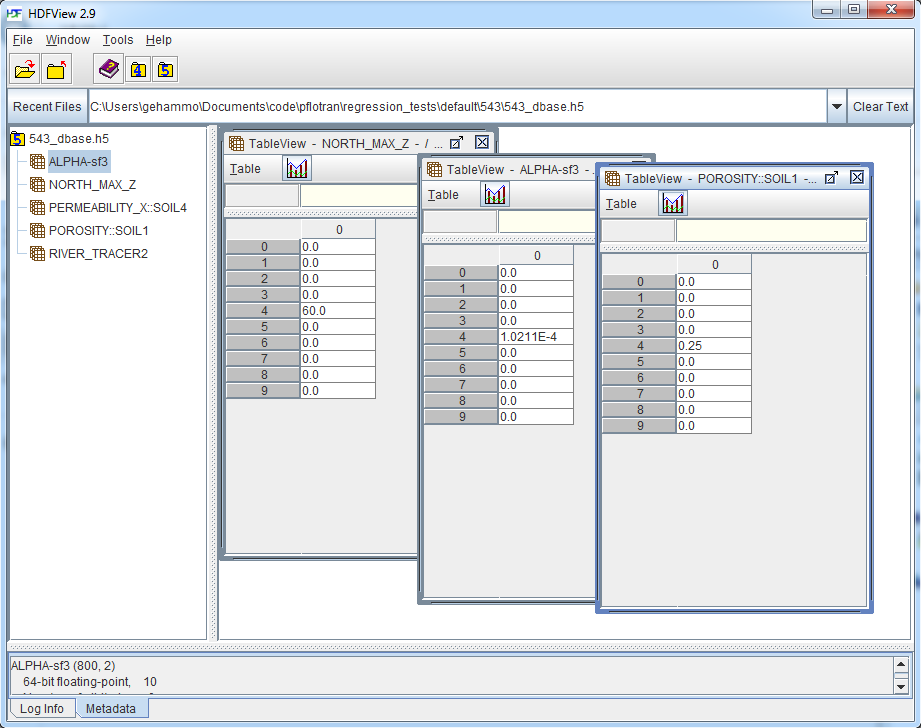
\includegraphics[scale=0.65]{./figs/h5_dbase.png}
\end{center}

\hyperlink{target_key}{\return}

%========================================================================

\newpage
\protect\hypertarget{target_dbg}{}

\subsection{Keyword: DEBUG}

{\noindent\bf Input:}
\begin{deflist}{00}
\item[DEBUG]~
\begin{deflist}{00}
\item[PRINT\_SOLUTION] [\bf VECVIEW\_SOLUTION, VIEW\_SOLUTION]
\item[PRINT\_RESIDUAL] [VECVIEW\_RESIDUAL,VIEW\_RESIDUAL]
\item[PRINT\_JACOBIAN] [MATVIEW\_JACOBIAN, VIEW\_JACOBIAN]
\item[PRINT\_JACOBIAN\_NORM] [NORM\_JACOBIAN]
\item[PRINT\_COUPLERS] [PRINT\_COUPLER]
\item[PRINT\_JACOBIAN\_DETAILED] [MATVIEW\_JACOBIAN\_DETAILED, 

VIEW\_JACOBIAN\_DETAILED]

\item[PRINT\_NUMERICAL\_DERIVATIVES] [VIEW\_NUMERICAL\_DERIVATIVES]

\end{deflist}
\item[\keyend]
\end{deflist}

{\noindent\bf Explanation:}

\bigskip

\begin{mdframed}

{\noindent\bf Examples:}
\begin{verbatim}
DEBUG
  PRINT_RESIDUAL
  PRINT_JACOBIAN
END
\end{verbatim}
\end{mdframed}

\hyperlink{target_key}{\return}

%================================================================

\newpage
\protect\hypertarget{target_eos}{}

\subsection{Keyword: EOS}

The {\bf EOS} keyword defines an equation of state for a simulated fluid.

%Required Cards:
\begin{deflist}{000}
%\item EOS <string>
\item[EOS] \ <string> \ [WATER, GAS] \ Specifies the fluid for which EOS applies.

{\bf Optional Input:}

\begin{deflist}{000}
\item[DENSITY] \ <string> \ <optional parameters>
\begin{deflist}{000}
\item[DENSITY CONSTANT] \ <float>
\item[DENSITY EXPONENTIAL] \ <float> <float> <float> \ (ref. density [rho0], ref. pressure [p0], compressibility) 
$\rho = \rho_0 \e^{\kappa (p-p_0)}$.

%Exponential function: rho0 * exp(compressibility*(pressure - p0))
\item[DENSITY DEFAULT] \ 
Default water EOS based on International Formulation Committee of the Sixth International Conference on Properties of Steam (1967)
\item[ENTHALPY] \ <string> \ <optional parameters>
\item[ENTHALPY CONSTANT] \ <float>
\item[VISCOSITY] \ <string> \ <optional parameters>
\end{deflist}
\end{deflist}
\item[\keyend] ~
\end{deflist}

\begin{mdframed}

{\noindent\bf Examples:}
\begin{verbatim}
EOS WATER
  DENSITY EXPONENTIAL 997.16d0 101325.d0 1.d-8
END
EOS WATER
  DENSITY CONSTANT 997.16d0
  ENTHALPY CONSTANT 1.8890d0
  VISCOSITY CONSTANT 8.904156d-4
END
\end{verbatim}
\end{mdframed}

\hyperlink{target_key}{\return}

%================================================================

\newpage
\protect\hypertarget{target_flow_cond}{}

\subsection{Keyword: FLOW\_CONDITION}

{\noindent\bf Description:}
The {\bf FLOW\_CONDITION} keyword specifies scalar or vector data sets to be associated with a given boundary or initial condition.  For instance, to specify a hydrostatic boundary condition, the use would specify a condition with a pressure associated with a point in space (i.e. datum) in space and a gradient, both vector quantities.  Note that in the case of a hydrostatic boundary condition, the vertical gradient specified in the input deck must be zero in order to enable the hydrostatic pressure calculation.  Otherwise, the specified vertical gradient overrides the hydrostatic pressure.  Transient pressures, temperatures, concentrations, datums, gradients, etc. are specified using the {\bf FILE} {\tt filename} combination for the name of the data set.

{\noindent\bf Input:}
\begin{deflist}{000}
\item [FLOW\_CONDITION] \ {\tt flow\_condition\_name}
\begin{deflist}{000}
\item [UNITS] {\tt <char>} (not currently supported)
\begin{deflist}{000000000}
{\tt <char>} is one of the following entries:
\item[s, min, h (hr), d, day, w, week, mo, month, y (yr)] (time)
\item[mm, cm, m, dm, km] (length)
\item[kg/s, kg/yr] (rate)
\item[Pa, KPa] (pressure)
\item[m/s, m/yr] (velocity)
\item[C, K] (temperature)
\item[M, mol/L] (concentration)
\item[KJ/mol] (enthalpy)
\end{deflist}

%\item[\keyend]

\item[CYCLIC] 

\item[INTERPOLATION] ~
\begin{deflist}{000}
\item[step]
\item[linear]
\end{deflist}

\item[SYNC\_TIMESTEP\_WITH\_UPDATE] ~

\item[TYPE] ~

\begin{deflist}{000000}
\item[PRESSURE] {\tt [dirichlet, hydrostatic, zero\_gradient, conductance,  \linebreak seepage]}
\item[RATE] \ {\tt [mass\_rate, volumetric\_rate, scaled\_volumetric\_rate]}: \ specifies an injection/extraction rate in mass [kg/s], volume [m$^3$/s], and a volumetric injection/extraction rate [m$^3$/s] that is scaled across a well screen, weighted as a function of the interfacial area and permeability of neighboring cells (in $x$, $y$).

\item[FLUX] {\tt [dirichlet, neumann, mass\_rate, hydrostatic, conductance,  \linebreak zero\_gradient, production\_well, seepage, volumetric, \linebreak volumetric\_rate, equilibrium]}
\item[TEMPERATURE] {\tt [dirichlet, hydrostatic, zero\_gradient]}
\item[CONCENTRATION] {\tt [dirichlet, hydrostatic, zero\_gradient]}
\item[SATURATION] {\tt [dirichlet]}
\item[ENTHALPY (H)] {\tt [dirichlet, hydrostatic, zero\_gradient]}
\end{deflist}
\item[\keyend]
\item[TIME] (not currently supported)

\item[IPHASE] {\tt <int>}

\item[DATUM] ~
\begin{deflist}{000}
\item[{\tt x \ y \ z}]
\item[{\bf FILE} \ {\tt file\_name}]
\end{deflist}
\item[GRADIENT, GRAD] ~
\begin{deflist}{000}
\item [PRES, PRESS, PRESSURE] ~
\begin{deflist}{000}
\item[$d_{dx}$ $d_{dy}$ $d_{dz}$]
\item[{\bf FILE} \ {\tt file\_name}]
\end{deflist}
\item [FLUX]
\item [TEMP, \ TEMPERATURE]
\item [CONC, \ CONCENTRATION]
\item [H, \ ENTHALPY]
\end{deflist}
\item[\keyend]
\item[TEMPERATURE, \ TEMP] \ {\tt <float>}
\item[ENTHALPY, H] \ {\tt <float>}
\item[PRESSURE, \ PRES, \ RESS] \ {\tt <float>}
\item[RATE] \ {\tt <float>}
\item[FLUX, \ VELOCITY, \ VEL] \ {\tt <float>}
\item[CONC, \ CONCENTRATION] \ {\tt <float>}
\item[SAT, \ SATURATION] \ {\tt <float>}
\item[CONDUCTANCE] \ {\tt <float>}
%\item[CONSTRAINT\_LIST]
\end{deflist}
\item[\keyend] ~
\end{deflist}

{\noindent\bf Explanation:}

\begin{center}
\begin{tabular}{ccc}
IPHASE & Phases present & CO$_2$ concentration\\
1 & H$_2$O & $X_{\rm CO_2}^{\rm H_2O}$\\
2 & SC CO$_2$ & $X_{\rm CO_2}^{\rm SC CO_2}$\\
3 & H$_2$O -- SC CO$_2$ & \Big($X_{\rm CO_2}^{\rm H_2O}\Big)_{\rm eq}$\\
\end{tabular}
\end{center}

\begin{center}
\begin{tabularx}{\linewidth}{lX}
\toprule[1.5pt]
\bf Keyword & \bf Description\\
\midrule
\bf FLOW/TRANSPORT\_CONDITION & Initiates a condition entry and defines its name\\
\midrule
\bf CYCLIC & Instructs PFLOTRAN to cycle the transient data set should the simulation time exceed the last time in the data set\\
\midrule
\bf INTERPOLATION & Defines the method for interpolating between data set times\\
\midrule
\bf SYNC\_TIMESTEP\_WITH\_UPDATE & Synchronizes time step with waypoints\\
\midrule
\bf DATUM & Location is space where prescribed scalar (e.g. pressure, temperature concentration, etc.) is defined\\
\midrule
\bf TYPE & Specifies condition type\\
\midrule
\bf PRESSURE & Specifies pressure condition type\\
 \bf TEMPERATURE & Specifies temperature condition type\\
    \bf CONCENTRATION & Specifies the type of concentration condition\\
    \bf SATURATION & Specifies saturation condition type\\
    \bf ENTHALPY & Specifies enthalpy condition type\\
    \bf END & Terminates type entry\\
\toprule[1.5pt]
\bf GRADIENT & Gradient of the scalar field in 3D space\\
\midrule
\bf PRESSURE & Pressure gradient in $x$-, $y$-, and $z$-directions\\
\bf TEMPERATURE & Temperature gradient in $x$-, $y$-, and $z$-directions\\
\bf CONCENTRATION & Concentration gradient in $x$-, $y$-, and $z$-directions\\
\bf ENTHALPY & Enthalpy gradient in $x$-, $y$-, and $z$-directions\\
\bf END & Terminates gradient entry\\
\toprule[1.5pt]
\bf PRESSURE & Absolute fluid pressure at the datum\\
\bf FLUX & Darcy velocity of fluid defining flux across specified boundary\\
\bf TEMPERATURE & Temperature in $^\circ$C at datum\\
\bf CONCENTRATION & Solute concentration at datum\\
\bf SATURATION & Solute saturation at datum\\
\bf ENTHALPY & Enthalpy at datum\\
\bf CONSTRAINT\_LIST & Specifies list of concentration constraints for solute transport\\
\bf END & Terminates condition entry\\
\bottomrule[1.5pt]
\end{tabularx}
\end{center}

\bigskip

\begin{mdframed}

{\noindent\bf Examples:}
\footnotesize
\begin{verbatim}
FLOW_CONDITION initial
  TYPE
    PRESSURE hydrostatic
  /
  PRESSURE 1956741.84 ! 200 meter piezometric head (200*997.32*9.81)
END

FLOW_CONDITION source
  TYPE
    RATE volumetric_rate
  /
  RATE 10. m^3/hr
END

TRANSPORT_CONDITION initial
  TYPE zero_gradient
  CONSTRAINT_LIST
    0.d0 initial
  /
END

TRANSPORT_CONDITION source
  TYPE dirichlet
  CONSTRAINT_LIST
    0.d0 well
  /
END

FLOW_CONDITION East
  TYPE
    :PRESSURE seepage
    PRESSURE conductance
  /
  CYCLIC
  DATUM file ../../river_scope3.datum
  GRADIENT
    PRESSURE file ../../river_scope3.gradient
  /
  CONDUCTANCE 1.d-12
  PRESSURE 101325.d0
END
\end{verbatim}
\end{mdframed}

\normalsize

\hyperlink{target_key}{\return}

%========================================================================

\newpage
\protect\hypertarget{target_fluid_property}{}

\subsection{Keyword: FLUID\_PROPERTY}

\noindent{\bf Description:} Assign diffusion coefficients and temperature dependence.

\noindent{\bf Input:}
\begin{deflist}{000}
\item[FLUID\_PROPERTY]~
\begin{deflist}{000}
\item[PHASE] \ {\tt <name>} \ (LIQUID\_PHASE, GAS\_PHASE) [Default: LIQUID\_PHASE]
\item[DIFFUSION\_COEFFICIENT] \ {\tt <float> [m$^2$/s]} [Default: $0\times 10^{-9}$ m$^2$/s]
\item[DIFFUSION\_ACTIVATION\_ENERGY] {\tt <float> [kJ/mol]} [Default: 0 kJ/mol]
\end{deflist}
\item[\keyend]
\end{deflist}

\noindent{\bf Explanation:} Read in reference diffusion coefficient $D_m^\circ$ and diffusion activation energy $A_D$. Temperature dependence of diffusion coefficient is calculated from the expression:
\EQ
D_m(T) \eq D_m^\circ\exp\Big[\frac{A_D}{R}\Big(\frac{1}{T_0} -\frac{1}{T}\Big)\Big],
\EN
where $D_m^\circ$ is the reference diffusion coefficient at temperature $T_0 = 25$\degc\ and $A_D$ denotes the diffusion activation energy.

\begin{mdframed}

\noindent{\bf Example:}
\begin{verbatim}
FLUID_PROPERTY
  DIFFUSION_COEFFICIENT 1.d-9      ! m^2/s
  DIFFUSION_ACTIVATION_ENERGY 12.6 ! kJ/mol
/
\end{verbatim}
\end{mdframed}

\hyperlink{target_key}{\return}

%========================================================================

\newpage
\protect\hypertarget{target_geomech}{}
 
\subsection{Keyword: GEOMECHANICS}

\noindent{\bf Description:} This keyword is required when using geomechanics. All the geomechanics part should go in this card.

\begin{description}
\item[GEOMECHANICS]~
\item[Required Input Parameters:]~
All the geomechanics keywords  should go here.
\item[\keyend] ~

\end{description}
%
%========================================================================

\newpage
\protect\hypertarget{target_geomech_grid}{}
 
\subsection{Keyword: GEOMECHANICS\_GRID}

\noindent{\bf Description:} The grid type and the format for geomechanics is specified here.
Only unstructured grids can be read. If you need to use a structured grid, generate the grid as an unstructured grid in the implicit format (see GRID keyword for details of the format below).

\begin{description}
\item[GEOMECHANICS\_GRID]~
\item[Required Input Parameters:]~

\begin{description}
\item[TYPE <type> :] ~

\begin{description}
\item Grid type (unstructured)
\end{description}

\item[FILE <filename>:] Name of file containing grid information (unstructured only)

\end{description}

\item[Optional Input Parameters:]~
\begin{description}
\item[GRAVITY] <\# \# \#>: Specifies gravity vector for geomechanics calculations (or specific body force) [Default: 0 0 -9.81 m/s$^2$] 
\end{description}


\item[\keyend] ~

\end{description}
%========================================================================

\newpage
\protect\hypertarget{target_geomech_output}{}
 
\subsection{Keyword: GEOMECHANICS\_OUTPUT}

\noindent{\bf Description:} This keyword is required for output of geomechanics data. The geomechanics data is saved in separate set of files (unlike flow and transport). The filenames of these files have the word \texttt{-geomech-} included in them.  Uses the same keywords as OUTPUT. 
%========================================================================

\newpage
\protect\hypertarget{target_geomech_material_prop}{}
 
\subsection{Keyword: GEOMECHANICS\_MATERIAL\_PROPERTY}
\noindent{\bf Description:} Specifies geomechanics material properties to be associated with a geomechanics region in the problem domain.

\noindent{\bf Input:}
\begin{deflist}{000}
\item[GEOMECHANICS\_MATERIAL\_PROPERTY] \ {\tt <char>}
\begin{deflist}{000}
\item[ID] \ {\tt <int>}
\item[YOUNGS\_MODULUS] \ {\tt <float>} \ [Pa]
\item[POISSONS\_RATIO] \ {\tt <float>}
\item[ROCK\_DENSITY] \ {\tt <float>} \ [kg/m$^3$]
\item[BIOT\_COEFFICIENT] \ {\tt <float>} 
\item[THERMAL\_EXPANSION\_COEFFICIENT] \ {\tt <float>} \ [Pa/K]
\end{deflist}
\item[\keyend]
\end{deflist}

\noindent{\bf Explanation:} The Young's modulus and Poisson's ratio (for the linear elastic model), rock density (used in body force calculation), Biot's coefficient and thermal expansion coefficient can be set here.

\begin{mdframed}

\noindent{\bf Example:}
\begin{verbatim}
MATERIAL_PROPERTY rock	 
  ID 1
  YOUNGS_MODULUS 1.d10
  POISSONS_RATIO 0.3
  ROCK_DENSITY 2200
  BIOT_COEFFICIENT 1.0
  THERMAL_EXPANSION_COEFFICIENT 1.d-5
END
\end{verbatim}

\end{mdframed}

\hyperlink{target_key}{\return}


%========================================================================

\newpage
\protect\hypertarget{target_geomech_region}{}
 
\subsection{Keyword: GEOMECHANICS\_REGION}

\noindent{\bf Description:} The GEOMECHANICS\_REGION keyword defines a set of geomechanics finite element grid vertices.
 The GEOMECHANICS\_REGION name can then be used to link this set of vertices to geomechanics  material properties, strata and boundary conditions. 
The list of vertices can be read from an ASCII file by using the keyword FILE under the GEOMECHANICS\_REGION card.

\begin{mdframed}

{\noindent\bf
Examples:}

\begin{verbatim}
GEOMECHANICS_REGION top 
  FILE top.vset 
END
\end{verbatim}

\end{mdframed}

\hyperlink{target_key}{\return}

%========================================================================

\newpage
\protect\hypertarget{target_geomech_condition}{}
 
\subsection{Keyword: GEOMECHANICS\_CONDITION}

\noindent{\bf Description:} Condition coupler between regions and geomechanics boundary conditions. Since the geomechanics is solved in a quasi-steady manner, initial conditions are not needed. 


{\noindent\bf Input:}
\begin{deflist}{000}
\item [GEOMECHANICS\_CONDITION] \ {\tt geomechanics\_condition\_name}
\begin{deflist}{000}
\item[TYPE] ~

\begin{deflist}{000000}
\item[DISPLACEMENT\_X] {\tt [dirichlet]}
\item[DISPLACEMENT\_Y] {\tt [dirichlet]}
\item[DISPLACEMENT\_Z] {\tt [dirichlet]}
\item[FORCE\_X] {\tt [dirichlet]}
\item[FORCE\_Y] {\tt [dirichlet]}
\item[FORCE\_Z] {\tt [dirichlet]}
\end{deflist}
\item[\keyend]
\item[DISPLACEMENT\_X] \ {\tt <float>}
\item[DISPLACEMENT\_Y] \ {\tt <float>}
\item[DISPLACEMENT\_Z] \ {\tt <float>}
\item[FORCE\_X] \ {\tt <float>}
\item[FORCE\_Y] \ {\tt <float>}
\item[FORCE\_Z] \ {\tt <float>}
\end{deflist}
\item[\keyend] ~
\end{deflist}

{\noindent\bf Explanation:}

\begin{center}
\begin{tabularx}{\linewidth}{lX}
\toprule[1.5pt]
\bf Keyword & \bf Description\\
\midrule
\bf GEOMECHANICS\_CONDITION & Initiates a geomechanics condition entry and defines its name\\
\midrule
\bf TYPE & Specifies condition type\\
\midrule
    \bf DISPLACEMENT\_X & Specifies $x-$ displacement condition type\\
    \bf DISPLACEMENT\_Y & Specifies $y-$ displacement condition type\\
    \bf DISPLACEMENT\_Z & Specifies $z-$ displacement condition type\\
    \bf FORCE\_X & Specifies in $x-$ force condition type\\
    \bf FORCE\_Y & Specifies in $y-$ force condition type\\
    \bf FORCE\_Z & Specifies in $z-$ force condition type\\
    \bf END & Terminates type entry\\
\toprule[1.5pt]
\bf DISPLACEMENT\_X & Displacement in the $x-$ direction \\ 
\bf DISPLACEMENT\_Y & Displacement in the $y-$ direction \\ 
\bf DISPLACEMENT\_Z & Displacement in the $z-$ direction \\ 
\bf FORCE\_X & Force in the $x-$ direction \\ 
\bf FORCE\_X & Force in the $y-$ direction \\ 
\bf FORCE\_X & Force in the $z-$ direction \\ 
\bf END & Terminates condition entry\\
\bottomrule[1.5pt]
\end{tabularx}
\end{center}


\begin{mdframed}

\noindent{\bf Example:}

\begin{verbatim}
GEOMECHANICS_CONDITION
  TYPE
    DISPLACEMENT_Z dirichlet
  /
DISPLACEMENT_Z 0.d0
END

\end{verbatim}
\end{mdframed}

\hyperlink{target_key}{\return}


%========================================================================

\newpage
\protect\hypertarget{target_geomech_bc}{}
 
\subsection{Keyword: GEOMECHANICS\_BOUNDARY\_CONDITION}

\noindent{\bf Description:} 
The GEOMECHANICS\_BOUNDARY\_CONDITION keyword couples condition specified under the GEOMECHANICS\_CONDITION keyword to a REGION in the problem domain.  The use of this keyword enables the use/reuse of geomechanics conditions and regions within multiple geomechanics boundary conditions the input deck.

{\noindent\bf Input:}

\begin{deflist}{000}
\item[GEOMECHANICS\_BOUNDARY\_CONDITION] {\tt geomechanics\_boundary\_condition\_name}
\begin{deflist}{000}
\item[GEOMECHANICS\_CONDITION] {\tt GEOMECHANICS\_condition\_name}
\item[REGION] {\tt region\_name}
\end{deflist}
\item[\keyend]
\end{deflist}

{\noindent\bf Explanation:}

\begin{center}
\begin{tabularx}{\linewidth}{lX}
\toprule[1.5pt]
\bf Keyword & \bf Description\\
\midrule
\bf GEOMECHANICS\_BOUNDARY\_CONDITION & Defines the beginning of a geomechanics boundary condition entry and the name of the geomechanics boundary condition.\\
\midrule
\bf GEOMECHANICS\_CONDITION & Defines the name of the geomechanics condition to be linked to this geomechanics boundary condition.\\
\midrule
\bf REGION & Defines the name of the region to which the conditions are linked.\\
\midrule
\bf END & Terminates the geomechanics boundary condition entry.\\
%\midrule\midrule
\bottomrule[1.5pt]
\end{tabularx}
\end{center}


\begin{mdframed}

\noindent{\bf Example:}

\begin{verbatim}
GEOMECHANICS_BOUNDARY_CONDITION bottom
  GEOMECHANICS_CONDITION z_disp_zero
  GEOMECHANICS_REGION bottom
END

\end{verbatim}
\end{mdframed}

\hyperlink{target_key}{\return}


%========================================================================

\newpage
\protect\hypertarget{target_geomech_strata}{}
 
\subsection{Keyword: GEOMECHANICS\_STRATA}

\noindent{\bf Description:} 
Couples geomechanics material IDs and/or properties with a geomechanics region in the problem domain.

\begin{deflist}{00}
\item[GEOMECHANICS\_STRATA] ~
\begin{deflist}{000}
\item[GEOMECHANICS\_MATERIAL] <string> \ name of the geomechanics material property to be associated with a geomechanics region
\item[GEOMECHANICS\_REGION] <string> \ name of geomechanics region associated with a geomechanics material property
\end{deflist}
\item[\keyend]
\end{deflist}

\begin{mdframed}
\noindent{\bf Example:}
\begin{verbatim}
GEOMECHANICS_STRATA
  GEOMECHANICS_MATERIAL granite 
  GEOMECHANICS_REGION all
END
\end{verbatim}
\end{mdframed}


%========================================================================

\newpage
\protect\hypertarget{target_grid}{}

\subsection{Keyword: GRID \hfill Required}

\noindent{\bf Description:} this keyword defines the descritization scheme, the type of grid and resolution, and the geometry employed in the simulation.

\begin{description}
\item[GRID]~
\item[Required Input Parameters:]~

\begin{description}
\item[TYPE <type> <symmetry>:] ~

\begin{description}
\item Grid type (structured, structured\_mimetic, unstructured, amr)

\item Symmetry type (cartesian [default], cylindrical, spherical)
\end{description}

\item[NXYZ <\# \# \#>:] \# of grid cells in $x$, $y$, $z$ directions (structured only)

\item[FILE <filename>:] Name of file containing grid information (unstructured only)

~\\

\noindent
\item[BOUNDS:] ~
\begin{description}
\item[<x\_min, \ y\_min, \ z\_min>]~
\item[<x\_max, \ y\_max, \ z\_max>]~
\end{description}
\item[\keyend] ~

~\\

\item[DXYZ:] Specifies grid spacing of structured cartesian grid (see examples below)
\begin{description}
\item[<{\bf dx}>] ~
\item[<{\bf dy}>] ~
\item[<{\bf dz}>] ~
\end{description}
\item[\keyend] ~
\end{description}

\item[Optional Input Parameters:] ~

\begin{description}

\item[GRAVITY <\# \# \#>:] Specifies gravity vector [Default: 0 0 $-$9.8068 m/s$^2$]

\item[ORIGIN <\# \# \#>:] Coordinate of grid origin [Default: 0 0 0]

\item[INVERT\_Z:] Inverts the $z$-axis [Default: positive $z$ points downward]
\end{description}
\end{description}

\begin{mdframed}

\noindent
{\bf Format of unstructured grid file:}

Implicitly defined grid:
\footnotesize
\begin{verbatim}
! 
! type: H=hexahedron, T=tetrahedron, W=wedge, P=pyramid
! vertn(H) = 8
! vertn(T) = 4
! vertn(W) = 6
! vertn(P) = 5
! -----------------------------------------------------------------
! num_cells num_vertices  (integers)
! type vert1 vert2 vert3 ... vertn  ! for cell 1 (integers)
! type vert1 vert2 vert3 ... vertn  ! for cell 2
! ...
! ...
! type vert1 vert2 vert3 ... vertn  ! for cell num_cells
! xcoord ycoord zcoord ! coordinates of vertex 1 (real)
! xcoord ycoord zcoord ! coordinates of vertex 2 (real)
! ...
! xcoord ycoord zcoord ! coordinates of vertex num_vertices (real)
! -----------------------------------------------------------------
\end{verbatim}
\end{mdframed}

\normalsize

\begin{mdframed}

Explicitly defined grid:

\footnotesize
\begin{verbatim}
! Format of explicit unstructured grid file
! id_, id_up_, id_dn_ = integer
! x_, y_, z_, area_, volume_ = real
! definitions
! id_ = id of grid cell
! id_up_ = id of upwind grid cell in connection
! id_dn_ = id of downwind grid cell in connection
! x_ = x coordinate of cell center
! y_ = y coordinate of cell center
! z_ = z coordinate of cell center
! volume_ = volume of grid cell
! -----------------------------------------------------------------
! CELLS <integer>    integer = # cells (N)
! id_1 x_1 y_1 z_1 volume_1
! id_2 x_2 y_2 z_2 volume_2
! ...
! ...
! id_N x_N y_N z_N volume_N
! CONNECTIONS <integer>   integer = # connections (M)
! id_up_1 id_dn_1 x_1 y_1 z_1 area_1
! id_up_2 id_dn_2 x_2 y_2 z_2 area_2
! ...
! ...
! id_up_M id_dn_M x_M y_M z_M area_M
! -----------------------------------------------------------------
\end{verbatim}
\end{mdframed}

\normalsize

\begin{mdframed}

\noindent
{\bf Examples:}
\begin{verbatim}
GRID
  TYPE structured cylindrical
  NXYZ 512  1  32
  DXYZ
    2.d0
    1.d0
    2.d0
  /
END
\end{verbatim}

\begin{verbatim}
GRID
  TYPE structured
  NXYZ 512 1 32
  BOUNDS
    0. 0. 0.
    1024. 1. 64.
  /
END
\end{verbatim}
\end{mdframed}

\noindent
By using the {\tt BOUNDS} keyword, the model domain is specified in a grid-independent fashion and, as a result, the grid spacing may be changed by modifying the keyword {\tt NXYZ} only.

\hyperlink{target_key}{\return}

\hyperlink{target_input_file}{\returnb}

%========================================================================

\newpage
\protect\hypertarget{target_init}{}

\subsection{Keyword: INITIAL\_CONDITION}

\noindent{\bf Description:} Condition coupler between regions and flow and transport conditions.

\noindent{\bf Input:}
\begin{deflist}{000}
\item[INITIAL\_CONDITION] \ [{\tt Name}]
\begin{deflist}{000}
\item[REGION] {\tt region\_name}
\item[FLOW\_CONDITION] {\tt condition\_name}
\item[TRANSPORT\_CONDITION] {\tt condition\_name}
%\item[TYPE] [{\tt initial, boundary, source\_sink}]
%\item[FACE] \ {\bf [WEST, EAST, NORTH, SOUTH, BOTTOM, TOP]}
\end{deflist}
\item[\keyend] ~
\end{deflist}

\noindent{\bf Explanation:}

\begin{mdframed}

\noindent{\bf Example:}

\begin{verbatim}
:=========== condition couplers ==============
: initial condition
INITIAL_CONDITION
  FLOW_CONDITION gradient-north
  TRANSPORT_CONDITION Initial
  REGION all
END
\end{verbatim}
\end{mdframed}

\hyperlink{target_key}{\return}

%========================================================================
\newpage

\protect\hypertarget{Keyword: INTEGRAL\_FLUX}{}

\subsection{Keyword: INTEGRAL\_FLUX}

\noindent{\bf Description:} Sets up a surface through which fluxes of all primary dependent variables can be calculated.

Note: add keyword {\tt PERIODIC\_OBSERVATION} to {\tt OUTPUT} keyword to toggle printing of integral fluxes to a file with the suffix {\tt '*-int.dat'}.

\noindent{\bf Input:}
\begin{deflist}{000}

\item[INTEGRAL\_FLUX] \ <string [Optional]> \ 
Opens input block and associates a name with INTEGRAL\_FLUX. [Required]

\begin{deflist}{000}

\item[NAME] \  <string> \
Specifies a name that is associated with the integral fluxes in the \break {\tt '*-int.dat'} file. This name will overwrite any name specified with the INTEGRAL\_FLUX keyword. [Optional]

\item[COORDINATES] \ 
Opens a block listing coordinates $(x_1,\, y_1,\, z_1)$, $(x_2,\, y_2,\, z_2)$, defining the rectangle over which the flux is to be calculated. The coordinates must form a rectangular plane that is aligned with the coordinate axes. [Required]

\item[INVERT\_DIRECTION] \ 
Inverts the sign of the flux. For fluxes at upwind boundaries, influx will be negative. This has no impact on the actual flux values other than to change the sign of the flux. [Optional]
\end{deflist}

\item[\keyend] ~
\end{deflist}


\begin{mdframed}

\noindent{\bf Examples:}

\begin{verbatim}
INTEGRAL_FLUX flux_up_shaft
  COORDINATES
    25.d0 15.d0 300.d0
    35.d0 20.d0 300.d0
  /
/

INTEGRAL_FLUX
  NAME inflow
  COORDINATES
    0.d0 0.d0 0.d0
    0.d0 10.d0 5.d0
  /
  INVERT_DIRECTION
/
\end{verbatim}
\end{mdframed}

\hyperlink{target_key}{\return}

%========================================================================


\newpage
\protect\hypertarget{target_linsolv}{}

\subsection{Keyword: LINEAR\_SOLVER}

\noindent{\bf Description:}

\noindent{\bf Input:}
\begin{deflist}{000}
\item[LINEAR\_SOLVER] \ [{\bf TRAN, TRANSPORT / FLOW}]

\begin{deflist}{000}
\item[SOLVER\_TYPE (SOLVER, KRYLOV\_TYPE, KRYLOV, KSP, KSP\_TYPE)] ~

\begin{deflist}{000}
\item[NONE (PREONLY)]
\item[DIRECT] \ (LU decomposition)
\item[ITERATIVE] \ (Bi-CGStab (BCGS) and block Jacobi preconditioning with ILU[0] in each block)
\item[GMRES]
\item[FGMRES]
\item[BCGS] \ (BICGSTAB, BI-CGSTAB) 
\item[IBCGS] \ (IBICGSTAB, IBI-CGSTAB) \ (Improved BCGS)
\item[RICHARDSON]
\item[CG]
\end{deflist}

\item[PRECONDITIONER\_TYPE (PRECONDITIONER, PC, PC\_TYPE)] ~

\begin{deflist}{000}
\item[NONE (PCNONE)]
\item[ILU (PCILU)] 
\item[LU (PCLU)]
\item[BJACOBI (BLOCK\_JACOBI)]
\item[ASM (ADDITIVE\_SCHWARTZ)]
\item[PCASM]
\item[HYPRE]
\item[SHELL]
\end{deflist}

\item[HYPRE\_OPTIONS]
\begin{deflist}{000}
\item[TYPE] \ [{\tt pilut, parasails, boomeramg, euclid}]
\item[BOOMERAMG\_CYCLE\_TYPE] \ <char> \ [{\tt V, W}]
\item[BOOMERAMG\_MAX\_LEVELS] \ {\tt <int>}
\item[BOOMERAMG\_MAX\_ITER] \ {\tt <int>}
\item[BOOMERAMG\_TOL] \ {\tt <float>}
\item[BOOMERAMG\_TRUNCFACTOR] \ {\tt <float>}
\item[BOOMERAMG\_AGG\_NL] \ {\tt <float>}
\item[BOOMERAMG\_AGG\_NUM\_PATHS] \ {\tt <int>}
\item[BOOMERAMG\_STRONG\_THRESHOLD] \ {\tt <float>}
\item[BOOMERAMG\_GRID\_SWEEPS\_ALL] \ {\tt <float>}
\item[BOOMERAMG\_GRID\_SWEEPS\_DOWN] \ {\tt <float>}
\item[BOOMERAMG\_GRID\_SWEEPS\_UP] \ {\tt <float>}
\item[BOOMERAMG\_GRID\_SWEEPS\_COARSE] \ {\tt <float>}
\item[BOOMERAMG\_RELAX\_TYPE\_ALL] \ {\tt <Value>}
\item[BOOMERAMG\_RELAX\_TYPE\_DOWN] \ {\tt <Value>}
\item[BOOMERAMG\_RELAX\_TYPE\_UP] \ {\tt <Value>}
\item[BOOMERAMG\_RELAX\_TYPE\_COARSE] \ {\tt <Value>}
\item[BOOMERAMG\_RELAX\_WEIGHT\_ALL] \ {\tt <Value>}
\item[BOOMERAMG\_RELAX\_WEIGHT\_LEVEL] \ {\tt <Value>}
\item[BOOMERAMG\_OUTER\_RELAX\_WEIGHT\_ALL] \ {\tt <Value>}
\item[BOOMERAMG\_OUTER\_RELAX\_WEIGHT\_LEVEL] \ {\tt <Value>}
\item[BOOMERAMG\_NO\_CF] \ {\tt <Value>}
\item[BOOMERAMG\_MEASURE\_TYPE] \ {\tt <Value>}
\item[BOOMERAMG\_COARSEN\_TYPE] \ {\tt <Value>}
\item[BOOMERAMG\_INTERPOLATION\_TYPE, BOOMERAMG\_INTERP\_TYPE] \ {\tt <Value>}
\item[BOOMERAMG\_NODAL\_COARSEN] \ {\tt <Value>}
\item[BOOMERAMG\_NODAL\_RELAXATION] \ {\tt <Value>}
\end{deflist}

\item[ATOL] \ {\tt <float>} \ (Absolute tolerance: $||b-Ax_n|| < \epsilon$)
\item[RTOL] \ {\tt <float>} \ (Relative tolerance: $||b-Ax_n||/||b-Ax_0||<\epsilon$)
\item[DTOL] \ {\tt <float>} \ (Divergence tolerance: $||b-Ax_n||/||b-Ax_0||>\epsilon$)
\item[MAXIT] \ {\tt <int>} \ (Maximum number of linear solver iterations)
\item[LU\_ZERO\_PIVOT\_TOL] \ {\tt <float>} \ Specifies zero pivot tolerance for ILU/LU preconditioners

\end{deflist}
\item[\keyend]
\end{deflist}

\noindent{\bf Explanation:}

\begin{mdframed}

\noindent{\bf Examples:}
\begin{verbatim}
LINEAR_SOLVER FLOW
  SOLVER DIRECT
/

LINEAR_SOLVER TRANSPORT
  SOLVER ITERATIVE
/

LINEAR_SOLVER FLOW
  SOLVER GMRES
  PRECONDITIONER ILU
/
Advanced PETSc options

LINEAR_SOLVER FLOW
  KSP_TYPE IBCGS
  PC_TYPE ASM
/

LINEAR_SOLVER TRANSPORT
  KSP_TYPE PCNONE
  PC_TYPE LU
  LU_ZERO_PIVOT_TOL 1d-15
/
\end{verbatim}
\end{mdframed}

\hyperlink{target_key}{\return}

%========================================================================

\newpage
\protect\hypertarget{target_mat}{}

\subsection{Keyword: MATERIAL\_PROPERTY}

\noindent{\bf Description:} Specifies material properties to be associated with a region in the problem domain.

\noindent{\bf Input:}
\begin{deflist}{000}
\item[MATERIAL\_PROPERTY] \ {\tt <char>}
\begin{deflist}{000}
\item[ID] \ {\tt <int>}
\item[SATURATION\_FUNCTION] \ {\tt <char>}
\item[ROCK\_DENSITY] \ {\tt <float>} \ [kg/m$^3$]
\item[SPECIFIC\_HEAT] \ {\tt <float>} \ [J/kg/K]
\item[LONGITUDINAL\_DISPERSIVITY] \ {\tt <float>} \ [m]
\item[TRANSVERSE\_DISPERSIVITY] \ {\tt <float>} \ (not implemented) \ [m]
\item[THERMAL\_CONDUCTIVITY\_DRY] \ {\tt <float>} \ [W/m/K]
\item[THERMAL\_CONDUCTIVITY\_WET] \ {\tt <float>} \ [W/m/K]
\item[PORE\_COMPRESSIBILITY] \ {\tt <float>} \ (not implemented) \ [bar$^{-1}$]
\item[THERMAL\_EXPANSITIVITY] \ {\tt <float>} \ (not implemented) \ [C$^{-1}$]
\item[POROSITY] \ {\tt <float>} \ [---], {\tt porosity\_filename}
%\item[POROSITY] \ {\tt porosity\_filename}
\item[TORTUOSITY] \ {\tt <float>} \ [---]
\item[PERMEABILITY] ~
\begin{deflist}{000}
\item[ISOTROPIC] \ Toggles on isotropy [Default]
\item[ANISOTROPIC] \ Toggles on anisotropy
\item[VERTICAL\_ANISOTROPY\_RATIO] \ {\tt <float>}
\item[PERM\_X] \ {\tt <float>} \ Diagonal permeability $k_{xx}$ [m$^2$]
\item[PERM\_Y] \ {\tt <float>} \ Diagonal permeability $k_{yy}$ [m$^2$]
\item[PERM\_Z] \ {\tt <float>} \ Diagonal permeability $k_{zz}$ [m$^2$]
\item[PERM\_ISO] \ {\tt <float>} \ Isotropic permeability values [m$^2$]
\item[PERM\_XY] \ {\tt <float>} \ Off-diagonal permeability $k_{xy}$ for use with MFD \\(mimetic\_unstructured grid) [m$^2$] (not currently supported)
\item[PERM\_XZ] \ {\tt <float>} [m$^2$] \ Off-diagonal permeability $k_{xz}$
\item[PERM\_YZ] \ {\tt <float>} [m$^2$] \ Off-diagonal permeability $k_{yz}$
\end{deflist}
\item[\keyend]
\item[PERMEABILITY\_POWER] \ {\tt <float>} \ (see Eqn.\eqref{permeability})
\item[PERMEABILITY\_CRIT\_POR] \ {\tt <float>} \ (see Eqn.\eqref{permf})
\item[PERMEABILITY\_MIN\_SCALE\_FAC] \ {\tt <float>} \ (see Eqn.\eqref{fmin})
\item[TORTUOSITY\_POWER] \ {\tt <float>}
\item[MINERAL\_SURFACE\_AREA\_POWER] ~ toggle to update mineral surface area \\(see {\tt MINERAL\_KINETICS} keyword for setting porosity or volume fraction power)
%\begin{deflist}{000}
%\item[VOLUME\_FRACTION] \ {\tt <float>} \ Volume fraction power in mineral surface area
%\item[POROSITY] \ {\tt <float>} \ Porosity power in mineral surface area
%\end{deflist}
%\item[\keyend]
\item[SECONDARY\_CONTINUUM] \ Activate with {\tt MULTIPLE\_CONTINUUM} keyword 
\begin{deflist}{000}
\item[TYPE] \ {\tt <char>} (SLAB, NESTED\_CUBES, NESTED\_SPHERES)
\item[NUM\_CELLS] \ {\tt <int>} \ Number of secondary continuum grid cells
\item[LOG\_GRID\_SPACING] \ Toggle to use logarithmic grid spacing in secondary continua (applies to nested spheres and cubes only)
\item[OUTER\_SPACING] \ {\tt <float>} [m] \ Outer matrix node grid spacing for logarithmic grid \ (see Eqns.\eqref{eqnloggrid})
\item[LENGTH] \ {\tt <float>} [m] \ length of SLAB type
\item[AREA] \ {\tt <float>} [m$^2$] \ cross-section area for SLAB type
\item[MATRIX\_BLOCK\_SIZE] \ {\tt <float>} [m] \ matrix block size for NESTED\_CUBES type
\item[FRACTURE\_SPACING] \ {\tt <float>} [m] \ fracture spacing for NESTED\_CUBES type
\item[RADIUS] \ {\tt <float>} [m] \ radius for NESTED\_SPHERES type
\item[EPSILON] \ {\tt <float>} \ Volume fraction of the primary continuum (fracture) in REV
\item[APERTURE] \ {\tt <float>} \ Fracture aperture (if specified overrides epsilon---applicable for nested cubes only)
\item[AREA\_SCALING\_FACTOR] \ {\tt <float>} \ Factor multiplying primary-secondary continua coupling term (default set to 1)
\end{deflist}
\item[\keyend]
%\item[RANDOM\_DATASET] \ {\tt permeability\_filename}
\end{deflist}
\item[\keyend]
\end{deflist}

\noindent{\bf Explanation:}

\begin{mdframed}

\noindent{\bf Example:}
\begin{verbatim}
MATERIAL_PROPERTY  Hanford
  ID 1
  SATURATION_FUNCTION sf1
  POROSITY 0.332
  TORTUOSITY 1.
  PERMEABILITY
    PERM_X 1.d-12
    PERM_Y 1.d-12
    PERM_Z 1.d-12
  /
END
=============
MATERIAL_PROPERTY soil1
  ID 1 
  SATURATION_FUNCTION sf1
  POROSITY 0.1
  TORTUOSITY 1.
  PERMEABILITY
    PERM_X 1.d-13
    PERM_Y 1.d-13
    PERM_Z 1.d-13
  /
  SECONDARY_CONTINUUM
    TYPE  SLAB
    LENGTH 50
    AREA 2500
    NUM_CELLS 10
    EPSILON 0.02
  /
END
\end{verbatim}

\noindent
{\bf Example: reading from a file for multiple realization simulation}

{\scriptsize\tt mpirun -np 10000 ./pflotran -stochastic -num\_realizations 1000 -num\_groups 100}

\begin{verbatim}
PFLOTRAN input file:

:=================== material properties ===================
MATERIAL_PROPERTY rock
ID 1
POROSITY 0.381d0
TORTUOSITY 1.d-1
ROCK_DENSITY 2.65d3
SPECIFIC_HEAT 1.d3
THERMAL_CONDUCTIVITY_DRY 2.5
THERMAL_CONDUCTIVITY_WET 2.5 
SATURATION_FUNCTION sf2
PERMEABILITY
  ANISOTROPIC ! default is ISOTROPIC
  DATASET Permeability
/
/

DATASET Permeability
  FILENAME ./permeability_with_white_noise_multi.h5
  REALIZATION_DEPENDENT
/

\end{verbatim}
\noindent
Python script fragment to generate permeability field:
\begin{Verbatim}
dataset_name = 'PermeabilityX'
h5dset = h5file.create_dataset(dataset_name, data=rarray1)
print 'done with ', dataset_name

dataset_name = 'PermeabilityY'
h5dset = h5file.create_dataset(dataset_name, data=rarray2)
print 'done with ', dataset_name

dataset_name = 'PermeabilityZ'
h5dset = h5file.create_dataset(dataset_name, data=rarray3)
print 'done with ', dataset_name
\end{Verbatim}

\noindent
For the full permeability tensor the dataset naming convention is:
\begin{Verbatim}
PermeabilityX
PermeabilityY
PermeabilityZ
PermeabilityXY
PermeabilityXZ
PermeabilityYZ
\end{Verbatim}

\end{mdframed}

\hyperlink{target_key}{\return}
%\hyperlink{target_key}{\hfill$\hookrightarrow$}

%========================================================================

\begin{comment}
\newpage
\protect\hypertarget{target_max}{}

\subsection{Keyword: MAX\_CHANGE}

\noindent{\bf Description:}

\noindent{\bf Input:}
\begin{deflist}{000}
\item[MAX\_CHANGE] \ {\tt DPMAX} \ {\tt DTMAX} \ {\tt DSMAX} \ {\tt DCMAX}
\end{deflist}

\noindent{\bf Explanation:}

\begin{mdframed}

\noindent{\bf Example:}
\begin{verbatim}
:          dpmax dtmax dsmax dcmax
:geh - this is bogus!
MAX_CHANGE 5.d4    5.  0.02   0.05
/
/
\end{verbatim}
\end{mdframed}

\hyperlink{target_key}{\return}
\end{comment}

%========================================================================

\newpage
\protect\hypertarget{target_mode}{}

\subsection{Keyword: MODE}

\noindent{\bf Description:} determines the flow mode: Richards (variably saturated porous media); MPH, \linebreak MPHASE, FLASH2 (CO$_2$ + H$_2$O); TH (Thermal-Hydrologic); IMMIS, THS (Immisible).

\begin{comment}
\noindent{\bf Input:}
\begin{deflist}{000}
\item[MODE] <option>
\item[Options:] ~
\begin{deflist}{000}
\item[RICHARDS]
\item[MPHASE (MPH)]
\item[FLASH2]
\item[TH]
\item[IMMIS (IMS, THS)]
\end{deflist}
\end{deflist}
\end{comment}

%\noindent{\bf Explanation:}

%\begin{center}
\begin{tabularx}{\linewidth}{lX}
%\toprule[1.5pt]
\multicolumn{2}{c}{\bf MODE \ <option>}\\
%\midrule
\multicolumn{1}{c}{\bf Option} & \multicolumn{1}{c}{\bf Description}\\
%\midrule
\bf GENERAL & Two-phase air-water, nonisothermal, variably saturated groundwater flow\\
\bf RICHARDS & Single-phase, isothermal, variably saturated groundwater flow using Richards equation\\
%\midrule
\bf MPHASE (MPH) & Two-phase supercritical CO$_2$-brine-energy based on variable switching for phase changes\\
%\midrule
\bf FLASH2 & Two-phase supercritical CO$_2$-brine-energy based on the flash method for phase changes with a persistent set of unknowns\\
%\midrule
\bf TH & Thermal-Hydrologic coupled groundwater flow\\
%\midrule
\bf IMMIS (IMS, THS) & Immissible CO$_2$-water-energy\\
\bf MIS & Missible H$_2$O-glycol fluid\\
%\bottomrule[1.5pt]
\end{tabularx}
%\end{center}

\begin{mdframed}

\noindent{\bf Example:}
\begin{verbatim}
MODE TH
\end{verbatim}
\end{mdframed}

\hyperlink{target_key}{\return}

%========================================================================

\newpage
\protect\hypertarget{target_mc}{}

\subsection{Keyword: MULTIPLE\_CONTINUUM}

\noindent{\bf Description:} 
This keyword initiates the multiple continuum formulation (implemented currently only for heat equation). The properties of the secondary continuum can be
specified under the MATERIAL\_PROPERTY keyword.

\begin{tabularx}{\linewidth}{lX}
%\toprule[1.5pt]
\bf MULTIPLE\_CONTINUUM & Activate multiple continuum model for heat and single solute transport equation. 
\end{tabularx}

\hyperlink{target_key}{\return}

%========================================================================

\newpage
\protect\hypertarget{target_newt}{}

\subsection{Keyword: NEWTON\_SOLVER}

\noindent{\bf Description:} 

\noindent{\bf Input:}
\begin{deflist}{000}
\item[NEWTON\_SOLVER] ~
\begin{deflist}{000}
\item[TRAN, TRANSPORT (tran\_solver) / DEFAULT (flow\_solver)]
\item[INEXACT\_NEWTON]
\item[NO\_PRINT\_CONVERGENCE]
\item[NO\_INF\_NORM (NO\_INFINITY\_NORM)]
\item[NO\_FORCE\_ITERATION]
\item[PRINT\_DETAILED\_CONVERGENCE]
\item[ATOL] \ {\tt <Value>}
\item[RTOL] \ {\tt <Value>}
\item[STOL] \ {\tt <Value>}
\item[DTOL] \ {\tt <Value>}
\item[ITOL \ (INF\_TOL, \ ITOL\_RES, \ INF\_TOL\_RES)] \ {\tt <Value>}
\item[ITOL\_UPDATE \ (INF\_TOL\_UPDATE)] \ {\tt <Value>}
\item[ITOL\_SEC \ (ITOL\_RES\_SEC, \ INF\_TOL\_SEC)] \ {\tt <Value>} \ Checks the infinite norm of secondary continuum residual for convergence when using transport. (default set to 1.d-10)
\item[MAXIT] \ {\tt <Value>} \ Cuts time step if the number of iterations exceed this value
\item[MAXF] \ {\tt <Value>}
\item[MAX\_NORM] \ {\tt <Value>} \ Cuts time step if the convergence norm exceeds this value. 
\end{deflist}
\item[\keyend]
\end{deflist}

\noindent{\bf Explanation:}

\scriptsize
\begin{Verbatim}
typedef enum {/* converged */
    SNES_CONVERGED_FNORM_ABS         =  2, /* ||F|| < atol */
    SNES_CONVERGED_FNORM_RELATIVE    =  3, /* ||F|| < rtol*||F_initial|| */
    SNES_CONVERGED_SNORM_RELATIVE    =  4, /* Newton computed step size small; 
                                              || delta x || < stol || x ||*/
    SNES_CONVERGED_ITS               =  5, /* maximum iterations reached */
    SNES_CONVERGED_TR_DELTA          =  7,
    
              /* diverged */
    SNES_DIVERGED_FUNCTION_DOMAIN     = -1, /* the new x location passed the function is 
                                               not in the domain of F */
    SNES_DIVERGED_FUNCTION_COUNT      = -2,
    SNES_DIVERGED_LINEAR_SOLVE        = -3, /* the linear solve failed */
    SNES_DIVERGED_FNORM_NAN           = -4,
    SNES_DIVERGED_MAX_IT              = -5,
    SNES_DIVERGED_LINE_SEARCH         = -6, /* the line search failed */
    SNES_DIVERGED_INNER               = -7, /* inner solve failed */
    SNES_DIVERGED_LOCAL_MIN           = -8, /* || J^T b || is small, implies converged to 
                                               local minimum of F() */
    SNES_CONVERGED_ITERATING          =  0} SNESConvergedReason;
\end{Verbatim}
\normalsize

\noindent{\bf Example:}

\hyperlink{target_key}{\return}

%========================================================================

\newpage
\protect\hypertarget{target_nonuniform_vel}{}

\subsection{Keyword: NONUNIFORM\_VELOCITY}
\begin{deflist}{0000000000}
\item[NONUNIFORM\_VELOCITY] <file name>
\end{deflist}

{\bf Explanation:} Name of HDF5 file for specifying nonuniform velocities including boundary velocities. Only applies to structured grids. The velocity must be specified in SI units (m/s).

Internal velocities are specified for each cell corresponding to the downwind face and read in separately for $v_x$, $v_y$, and $v_z$.
Boundary velocities are read in at all cells for each boundary condition (cells not in boundary condition region are ignored, but need a value to be read nonetheless).  

A boundary condition may not wrap around a corner. Corner cells should be mapped to multiple boundary conditions with their boundary faces residing in different regions.  
%If the user creates a user defined list of cells/faces for a region, the boundary condition could wrap around a corner.
Below is an example python script for generating an HDF5 velocity file.

\begin{mdframed}
\underline{Python script for generating an HDF5 velocity file read by PFLOTRAN.}
\footnotesize
\begin{Verbatim}
import sys
import math
from h5py import *
import numpy
import random

filename = 'velocity.h5'
h5file = File(filename,mode='w')

nx = 100
ny = 2
nz = 2
nxXny = nx*ny
n = nx*ny*nz

iarray = numpy.zeros((n),'=i4')

# add cell ids to file
for i in range(n):
  iarray[i] = i+1
dataset_name = 'Cell Ids'
h5dset = h5file.create_dataset(dataset_name, data=iarray)

rarray = numpy.zeros((n),'=f8')

# x velocity
for i in range(n):
  rarray[i] = 3.171e-8
dataset_name = 'Internal Velocity X'
h5dset = h5file.create_dataset(dataset_name, data=rarray)

# y velocity
for i in range(n):
  rarray[i] = 0.
dataset_name = 'Internal Velocity Y'
h5dset = h5file.create_dataset(dataset_name, data=rarray)

# z velocity
dataset_name = 'Internal Velocity Z'
h5dset = h5file.create_dataset(dataset_name, data=rarray)

# west boundary velocity
i = 0
for index in range(n):
  rarray[index] = 0.
for k in range(nz):
  for j in range(ny):
    index = k*(nx*ny) + j*nx + i
    rarray[index] = 3.171e-8
dataset_name = 'West'
h5dset = h5file.create_dataset(dataset_name, data=rarray)

# east boundary
i = nx-1
for index in range(n):
  rarray[index] = 0.
for k in range(nz):
  for j in range(ny):
    index = k*(nx*ny) + j*nx + i
    rarray[index] = -3.171e-8
dataset_name = 'East'
h5dset = h5file.create_dataset(dataset_name, data=rarray)

h5file.close()
print('done with everything')
\end{Verbatim}
\end{mdframed}

\begin{mdframed}
{\bf Example: }

\begin{Verbatim}
NONUNIFORM\_VELOCITY velocity.h5
\end{Verbatim}
\end{mdframed}

\hyperlink{target_key}{\return}

%========================================================================

\newpage
\protect\hypertarget{target_numjac_flow}{}

\subsection{Keyword: NUMERICAL\_JACOBIAN\_FLOW}
\begin{deflist}{0000000000}
\item[NUMERICAL\_JACOBIAN\_FLOW] 
Uses numerically evaluated Jacobian for flow.
\end{deflist}

\hyperlink{target_key}{\return}


%========================================================================

\newpage
\protect\hypertarget{target_numjac_rxn}{}

\subsection{Keyword: NUMERICAL\_JACOBIAN\_RXN}
\begin{deflist}{0000000000}
\item[NUMERICAL\_JACOBIAN\_RXN]
Uses numerically evaluated Jacobian for reactions.
\end{deflist}

\hyperlink{target_key}{\return}


%========================================================================

\newpage
\protect\hypertarget{target_numjac_multi}{}

\subsection{Keyword: NUMERICAL\_JACOBIAN\_MULTI\_COUPLE}
\begin{deflist}{0000000000}
\item[NUMERICAL\_JACOBIAN\_MULTI\_COUPLE]
The contribution to the primary continuum Jacobian due to primary-secondary continua coupling term is numerically evaluated.
\end{deflist}

\hyperlink{target_key}{\return}

%========================================================================

\newpage
\protect\hypertarget{target_observation}{}

\subsection{Keyword: OBSERVATION}

{\noindent\bf Description:}
The OBSERVATION card specifies a location (REGION) at which flow and transport results (e.g. pressure, saturation, flow velocities, solute concentrations, etc.) will be monitored in the output.
The user must specify either a region or boundary condition to which the observation object is linked.  The velocity keyword toggles on the printing of velocities at a point in space.

\noindent{\bf Input:}
\begin{deflist}{000}
\item[OBSERVATION] ~
\begin{deflist}{000}
\item[BOUNDARY\_CONDITION] \ {\tt boundary condition name}
\item[REGION] \ {\tt region name}
\item[VELOCITY]
\item[AT\_CELL\_CENTER]
\item[SECONDARY\_TEMPERATURE]
\item[SECONDARY\_CONCENTRATION]
\item[SECONDARY\_MINERAL\_VOLFRAC]
\end{deflist}
\item[\keyend]
\end{deflist}

{\noindent\bf Explanation:}
\begin{description}
\item[Keyword OBSERVATION] initiates an observation point entry.
\item[Keyword REGION] (optional) defines the name of the region (usually a point in space) to which the observation point is linked.
\item[Keyword BOUNDARY\_CONDITION] (optional) specifies the name of a boundary condition to which the observation point is tied (e.g. to monitor fluxes across a boundary face).
\item[Keyword VELOCITY] (optional) toggles on the printing of Darcy velocities at the observation point.
\item[Keyword SECONDARY\_TEMPERATURE] (optional) toggles on the printing of the secondary continuum (matrix nodes) temperatures.
\item[Keyword SECONDARY\_CONCENTRATION] (optional) toggles on the printing of the secondary continuum (matrix nodes) concentration.
\item[Keyword SECONDARY\_MINERAL\_VOLFRAC] (optional) toggles on the printing of the secondary continuum (matrix nodes) mineral volume fraction.
\end{description}

\begin{mdframed}

{\noindent\bf Examples:}
\begin{verbatim}
OBSERVATION
  REGION well1
  VELOCITY
END

OBSERVATION
BOUNDARY_CONDITION river
END
\end{verbatim}
\end{mdframed}

\hyperlink{target_key}{\return}

%========================================================================

\newpage
\protect\hypertarget{target_orig}{}

\subsection{Keyword: ORIGIN (ORIG)}
\begin{deflist}{0000000000}
\item[ORIGIN (ORIG)] X\_DIRECTION \ \ Y\_DIRECTION \ \ Z\_DIRECTION
\end{deflist}

\hyperlink{target_key}{\return}

%========================================================================


\newpage
\protect\hypertarget{target_output}{}

\subsection{Keyword: OUTPUT}

\noindent {\bf Description:} The {\bf OUTPUT} keyword controls formatting and time of output.

\noindent {\bf Input:}

\begin{deflist}{000}
\item[OUTPUT] ~
\begin{deflist}{000}
\item[TIMES] {\tt Unit (s, min, h (hr), d, w, mo, y (yr))} \ \ \ {\tt <float>} 
\item[SCREEN \ OFF] \ suppress screen output
\item[SCREEN \ PERIODIC] {\tt <int>}: print to screen every <integer> time steps.
\item[PERIODIC \ TIME] {\tt <float>} \ {\tt Unit}
\item[PERIODIC \ TIMESTEP] {\tt <float>} \ {\tt Unit}
\item[PERIODIC\_OBSERVATION \ TIME] \ {\tt <float>} \ {\tt <unit>}: \ output the results at observation points and mass balance output at specified output times
\item[PERIODIC\_OBSERVATION \ TIMESTEP] \ {\tt <integer>}: \ output the results at observation points and mass balance output at specified time steps 
\item[NO\_PRINT\_INITIAL] \ the initial state of the system will not be printed to the output file if this card is activated
\item[NO\_PRINT\_FINAL] \ the final state of the system will not be printed to the output file if this card is activated
\item[PRINT\_COLUMN\_IDS] print column numbers in observation and mass balance output files

\item[FORMAT] \ <file format>: \ specify the snapshot in time file type. File formats available are: 

\begin{deflist}{000000}
\item[TECPLOT] ~
\begin{deflist}{0000000000}
\item[POINT] -TecPlot point format (requires a single processor)
\item[BLOCK] -TecPlot block format
\item[FEBRICK] -TecPlot finite element
\end{deflist}

\item[HDF5] ~
\begin{deflist}{0000000000}
\item[SINGLE\_FILE] -produces single HDF5 file {\tt pflotran.h5}
\item[MULTIPLE\_FILES \ [TIMES\_PER\_FILE]] -produces a separate HDF5 file for number of times specified by TIMES\_PER\_FILE [default 1]
\end{deflist}

\item[MAD] -(not supported)
\item[VTK] -VTK format
\end{deflist}

\item[VOLUME] -Output cell volume
\item[PERMEABILITY] -Output cell permeability
\item[POROSITY] -Output cell porosity
\item[FLUXES] -Output interface fluxes
\item[VELOCITY\_AT\_FACE] -Output interface velocities 
\item[~] -Structured grid: velocity outputted at internal faces only. Visualization support is available via XDMF.
\item[~] -Unstructured grid: velocity outputted for internal and boundary faces. Data is outputted in HDF5 format only with no visualization support via XDMF.
\item[VELOCITY\_AT\_CENTER] -Output cell-centered velocities (supported for structured and unstructured grids, applies to TecPlot and HDF5 output formats). Note that this is compatible only with TecPlot BLOCK format.

\item[MASS\_BALANCE:] \ output the mass balance of the system if this card is activated. It includes global mass balance as well as fluxes at all boundaries for water and chemical species specified for output in the CHEMISTRY card. For the MPHASE mode only global mass balances are provided including supercritical CO$_2$. Output times are controlled by {\tt PERIODIC\_OBSERVATION TIMESTEP and TIME}, and printout times.
\end{deflist}
\item[\keyend]
\end{deflist}

\noindent {\bf Explanation:}

\begin{center}
\begin{tabularx}{\linewidth}{lX}
OUTPUT: & keyword to control output.\\
TIMES: & list of output times.\\
SCREEN OFF: & turns off screen output\\
SCREEN PERIODIC: & controls screen output frequency.\\
PERIODIC TIME: & controls frequency of output times.\\
PERIODIC TIMESTEP: & controls frequency of output time steps.\\
PERIODIC\_OBSERVATION TIME: & frequency of output time.\\
PERIODIC\_OBSERVATION TIMESTEP: & frequency of output time step.\\
NO\_FINAL, NO\_PRINT\_FINAL: & \\
FORMAT TECPLOT POINT: & Tecplot POINT output, valid for 1D and 2D problems on a single processor core.\\
FORMAT TECPLOT BLOCK: & Tecplot BLOCK output for multi-processor core runs.\\
FORMAT HDF5: & HDF5 output format written to a .h5 file which can be read by VisIt and ParaView.\\
FORMAT MAD: & MAD (Method of Anchored Distributions) format.\\
FORMAT VTK: & VTK format which can be read by VisIt and ParaView.\\
UNIT: & time units of seconds (s), minutes (min), hours (h, hr), days (d), weeks (w), months (mo), and years (y, yr).\\
PERMEABILITY: & \\
POROSITY: & \\
FLUXES: & \\
VELOCITIES: & keyword to output velocities.\\
MASS\_BALANCE: & keyword to output global mass balances and boundary fluxes, both cumulative and instantaneous.
\end{tabularx}
\end{center}

The output in the mass balance file refers to global mass conservation. This output is described in detail for the {\tt MPHASE} mode. The total number of moles of the $i$th component in phase $\a$ is given as the integral over the entire computational domain (see Eqn.\eqref{mass_conservation_equation})
\EQ
N_i^\a \eq \int_V \varphi s_\a \eta_\a x_i^\a \, dV.
\EN
From the governing equations, Eqn.\eqref{mass_conservation_equation}, the time rate of change of the total number of moles of the $i$th component
\EQ
N_i = \sum_\a N_i^\a,
\EN
is given by
\BA
\frac{dN_i}{dt} &\eq \sum_\a \frac{dN_i^\a}{dt} \\
&\eq -\sum_\a \int_{\p V} \bF_i^\a\cdot\bdS + Q_i,
\EA
where the surface integral on the right hand side is over the flux flowing through the boundaries of the domain.
The surface averaged flux $\F_i$ is defined as
\EQ
\F_i^\a \eq -\int_{\p V} \bF_i^\a\cdot\bdS,
\EN
defined as positive for flow into and negative for flow out of the domain $V$.
Integrating the flux over time gives the cumulative flux $\overline\F_i^\a$
\EQ
\overline\F_i^\a \eq \int_0^t \F_i^\a \, dt',
\EN
and time integrated source/sink $\overline Q_i$
\EQ
\overline Q_i \eq \int_0^t Q_i\, dt'.
\EN
Global conservation of mass implies the equality
\EQ
N_i(t) \eq N_i(0) + \sum_\a \overline\F_i^\a + \overline Q_i.
\EN

The header for the {\tt MPHASE} mass balance file reads (for time in years, $l$=aqueous liquid phase, sc=supercritical CO$_2$):
\BA
t, \ \ \Delta t, & \ [y]\nonumber \\
N_{\rm H_2O}^{l}, \ \ N_{\rm CO_2}^{l}, \ \ \widetilde N_{\rm CO_2}^{l}, \ \ N_{\rm H_2O}^{\rm sc}, \ \ N_{\rm CO_2}^{\rm sc}, \ \ \widetilde N_{\rm CO_2}^{\rm sc}, & \ \text{[kmol]} \nonumber \\
\overline \F_{\rm H_2O}^{l}, \ \ 
\overline \F_{\rm CO_2}^{l}, \ \ 
\overline \F_{\rm H_2O}^{\rm sc}, \ \ 
\overline \F_{\rm CO_2}^{\rm sc}, & \ \text{[kmol]} \nonumber \\
\F_{\rm H_2O}^{l}, \ \ 
\F_{\rm CO_2}^{l}, \ \ 
\F_{\rm H_2O}^{\rm sc}, \ \ 
\F_{\rm CO_2}^{\rm sc}, & \ \text{[kmol/y]}\nonumber\\
\overline Q_{\rm H_2O}, \ \ \overline Q_{\rm CO_2}, & \ \text{[kmol]}\nonumber\\
Q_{\rm H_2O}, \ \ Q_{\rm CO_2}, & \ \text{[kmol/y]}
\EA
The quantity $\widetilde N_i^\a$ denotes the trapped component in phase $\a$ defined by
\EQ
\widetilde N_i^\a \eq \int_{V, \, s_\a < s_\a^0} \varphi s_\a \eta_\a x_i^\a \, dV,
\EN
where $s_\a^0$ denotes the residual saturation. There are as many rows of cumulative and instantaneous fluxes as there are boundaries and source/sinks.

\begin{mdframed}

\noindent {\bf Examples:}

\begin{verbatim}
OUTPUT
  !SCREEN PERIODIC 10
  !PERIODIC TIME 10 h
  PERIODIC_OBSERVATION TIMESTEP 1
  !times h 1.
  !PERIODIC_OBSERVATION TIME 50 h
  FORMAT TECPLOT POINT ! or BLOCK
  FORMAT HDF5
  VELOCITIES
  MASS_BALANCE
END
\end{verbatim}
\end{mdframed}

\hyperlink{target_key}{\return}

%========================================================================

\newpage
\protect\hypertarget{target_overwrite}{}

\subsection{Keyword: OVERWRITE\_RESTART\_TRANSPORT}
%\shadowbox{
%\begin{minipage}{6.5in}
\begin{deflist}{0000000000}
\item[OVERWRITE\_RESTART\_TRANSPORT] \{overwrite\_restart\_transport = .true.\}
\end{deflist}
%\end{minipage}
%}

Overwrites checkpointing values with values read in from the input file on restart.

\hyperlink{target_key}{\return}

%================================================================

\newpage
\protect\hypertarget{target_proc}{}

\subsection{Keyword: PROC}

\begin{deflist}{0000}
\item[PROC] <int int int> 
\item[Description:] The number of processor to be employed in each direction $x$, $y$, and $z$ (structured grids only). Default: let PETSc decide. {\em Warning: the product of the integers must be equal to the number of processor employed.}
\end{deflist}

\begin{mdframed}

\noindent {\bf Examples:}

{\tt PROC 100 10 10} \ \ \ \ \ ! 10,000 processes

{\tt PROC 2 2 2} \ \ \ \ \ ! 2$\times$2$\times$2 decomposition

{\tt PROC 1 1 8} \ \ \ \ ! Force decomposition in z direction only (1$\times$1$\times$8 decomposition).

\end{mdframed}

\hyperlink{target_key}{\return}

%========================================================================

\newpage
\protect\hypertarget{target_region}{}


\subsection{Keyword: REGION}

{\noindent\bf Description:}
The {\bf REGION} keyword defines a set of grid cells encompassed by a volume or intersected by a plane or point, or a list of grid cell ids.  The {\bf REGION} name can then be used to link this set of grid cells to material properties, strata, boundary and initial conditions, source sinks, observation points, etc.  Although a region may be defined though the use of (I, J, K) indices using the {\bf BLOCK} keyword, the user is encouraged to define regions either through {\bf COORDINATES} or lists read in from an HDF5 file in order to minimize the dependence of the input file on grid resolution.  In the case of the {\bf FILE} keyword, a list of grid cell ids is read from an HDF5 file where the {\tt region\_name} defines the HDF5 data set.  It should be noted that given a region defined by a plane or point shared by two grid cells (e.g. a plane defining the surface between two grid cells), {\bf PFLOTRAN} will select the upwind cell(s) as the region.

{\noindent\bf Input:}

\begin{deflist}{000}
\item[REGION] {\tt region\_name}
\begin{deflist}{000}
\item[FILE] \ {\tt file\_name}
\item[LIST] \ (to be implemented)
\item[FACE] \ {\tt face\_name}
\item[BLOCK] \ {\tt i1 \ i2 \ j1 \ j2 \ k1 \ k2}
\item[COORDINATE] \ {\tt x \ y \ z}
\item[COORDINATES] ~
\begin{deflist}{000}
\item[\tt x1 y1 z1]
\item[\tt x2 y2 z2]
\end{deflist}
\item[\keyend]
\end{deflist}
\item[\keyend]
\end{deflist}

{\noindent\bf Explanation:}
\begin{description}
\item[Keyword REGION] begins a region entry with name {\tt region\_name}.
\item[Keyword BLOCK] defines a volumetric, planar, or point region through IJK indices: i1 i2 j1 j2 k1 k2.
\item[Keyword COORDINATE] defines a point region through coordinates in 3D space.
\item[Keyword COORDINATES] Defines a volumetric, planar, or point region between two points in space.
\item[Keyword FILE] Defines an HDF5 file within which a dataset named
region\_name contains a list of grid cells corresponding to a region.
\item [Keyword FACE] Defines the face of the grid cell to which boundary conditions are connected where face\_name is one of WEST, EAST, NORTH, SOUTH, BOTTOM, TOP (structured grids only).
\item [Keyword END] Ends the region entry (can be one of . \ END).
\end{description}

\begin{mdframed}

{\noindent\bf
Examples:}

\begin{verbatim}
REGION source_zone
  BLOCK 3 5 15 16 2 3
END

REGION source_zone
  BLOCK 3 5 15 16 2 3
END

REGION west_boundary
  BLOCK 1 1 1 30 1 50
  FACE WEST
END

REGION source_zone
  COORDINATES
    50. 10. 10.
    60. 15. 15.
  /
END

REGION river_boundary
  FILE ./regions.h5
  FACE EAST
END

REGION well
  COORDINATE 50. 10. 10.
END

REGION well
  COORDINATE 50. 10. 10.
END

REGION west_boundary
  COORDINATES
    0. 0. 0.
    0. 10. 10.
  /
  FACE WEST
END
\end{verbatim}

\end{mdframed}

\hyperlink{target_key}{\return}

%========================================================================

\newpage
\protect\hypertarget{target_restart}{}

\subsection{Keyword: RESTART}
{\noindent\bf Description}

The RESTART card defines a checkpoint file from which the current simulation should be restarted.  If a time is specified after the file name, the initial simulation time is set to that time.

{\noindent\bf Input:}

%\shadowbox{
%\begin{minipage}{6.5in}
\begin{deflist}{000}
\item[RESTART] \ <restart\_file\_name> \ <restart\_time> \ <time\_units>
\end{deflist}
%\end{minipage}
%}

{\noindent\bf Explanation:}
\begin{description}
\item[Keyword RESTART] defines the checkpoint filename to be read in to restart a simulation at the specified time.
\end{description}

{\noindent\bf
Examples:}

\begin{mdframed}

\begin{verbatim}
: restart the simulation from the end of the previous /
  simulation, but set the time back to 0.

RESTART restart.chk 0.d0 y

: restart the program running from where it left off /
  when the file pflotran.chk3000 was printed

RESTART pflotran.chk3000

\end{verbatim}

\end{mdframed}

\hyperlink{target_key}{\return}

%========================================================================

\newpage
\protect\hypertarget{target_sat}{}

\subsection{Keyword: SATURATION\_FUNCTION}


\includegraphics[scale=0.25]{./figs/under-construction.png}

\noindent{\bf Description:} Currently being revised to use a common set of saturation and relative permeability functions across all modes. Check source code for up-to-date implementation.

\noindent{\bf Input:}
\begin{deflist}{000}
\item[SATURATION\_FUNCTION] \ {\tt Name}

\begin{deflist}{000}
\item[SATURATION\_FUNCTION\_TYPE] \ [{\bf VAN\_GENUCHTEN}, \ {\bf BROOKS\_COREY}, 

{\bf THOMEER\_COREY}, \ {\bf NMT\_EXP}, \ {\bf PRUESS\_1}, \ {\bf VAN\_GENUCHTEN\_PARKER}]

\item[PERMEABILITY\_FUNCTION\_TYPE] \ [{\bf MUALEM}, \ {\bf BURDINE}]
\item[RESIDUAL\_SATURATION] \ {\tt <Value>} \ \ MODES: RICHARDS, TH
\item[RESIDUAL\_SATURATION\_LIQUID] \ {\tt <Value>} \ \ MODES: MPHASE
\item[RESIDUAL\_SATURATION\_GAS] \ {\tt <Value>} 

MODES: MPHASE ({\bf VAN\_GENUCHTEN\_PARKER})

\item[LAMBDA] \ {\tt <Value>} [---]
\item[ALPHA] \ {\tt <Value>} [Pa$^{-1}$]
\item[MAX\_CAPILLARY\_PRESSURE] \ {\tt <Value>} [Pa]
\item[BETAC] \ {\tt <Value>} [---] (Only used in {\bf NMT\_EXP})
\item[POWER] \ {\tt <Value>} [---] (Only used in {\bf NMT\_EXP})
\end{deflist}
\item[\keyend]
\end{deflist}

\noindent{\bf Explanation:}

\begin{mdframed}

\noindent{\bf Example:}
\begin{verbatim}
SATURATION_FUNCTION sf1
  SATURATION_FUNCTION_TYPE VAN_GENUCHTEN
  RESIDUAL_SATURATION 0.1d0
  LAMBDA 2.67d0
  ALPHA 2.042d-4
  MAX_CAPILLARY_PRESSURE 1d8
END
\end{verbatim}

\end{mdframed}

\hyperlink{target_key}{\return}

%========================================================================

\newpage
\protect\hypertarget{target_src}{}

\subsection{Keyword: SOURCE\_SINK}
\begin{deflist}{000}
\item[SOURCE\_SINK] \ {\tt <name>}
\begin{deflist}{000}
\item[REGION] \ <region\_name> \ name of the region the source/sink term is applied to
\item[FLOW\_CONDITION] \ <condition\_name> \ name of the flow condition
\item[TRANSPORT\_CONDITION] \ <condition\_name> \ name of the transport condition
\end{deflist}
\item[\keyend]
\end{deflist}

\begin{mdframed}

\noindent{\bf Example:}
\begin{verbatim}
SOURCE_SINK Well_2-9_1
  FLOW_CONDITION Injection_1
  TRANSPORT_CONDITION Source
  REGION Well_2-9_1
END
\end{verbatim}

\end{mdframed}

\hyperlink{target_key}{\return}

%========================================================================

\newpage
\protect\hypertarget{target_strata}{}

\subsection{Keyword: STRATIGRAPHY (STRATA)}

Couples material IDs and/or properties with a region in the problem domain.

%\shadowbox{
%\begin{minipage}{6.5in}
\begin{deflist}{00}
\item[STRATIGRAPHY (STRATA)] ~
\begin{deflist}{000}
\item[MATERIAL] <string> \ name of the material property to be associated with a region
\item[REGION] <string> \ name of region associated with a material property
%\item  INACTIVE
\end{deflist}
\item[\keyend]
\end{deflist}
%\end{minipage}
%}

\noindent
Note: a filename can be provided instead of a material property name from which material IDs are read on a cell by cell basis. In this case there is no need for the {\tt REGION} keyword.

\noindent {\bf Examples:}

\begin{mdframed}
\noindent
Assign {\tt hanford\_unit} material properties to the region {\tt source\_zone}

\begin{verbatim}
STRATA
  MATERIAL hanford_unit
  REGION source_zone
/
\end{verbatim}

\noindent
Assign material properties through material IDs read from an HDF5 formatted file. In this case there is no need to specify a region as material IDs are assigned to the entire grid on a cell by cell basis.

\begin{verbatim}
STRATA
  MATERIAL ../../field_material_ids.h5
/
\end{verbatim}

\noindent For a detailed example on creating the .h5 file see the PFLOTRAN wiki: \href{https://bitbucket.org/pflotran/pflotran-dev/wiki/Documentation/Strata}{Strata}.
\end{mdframed}

\hyperlink{target_key}{\return}

%========================================================================

\newpage
\protect\hypertarget{target_time}{}

\noindent {\bf Description:} the keyword {\bf TIME} controls the simulation time.

\noindent {\bf Input:}
\subsection{Keyword: TIME}
\begin{deflist}{000}
\item[TIME] ~
\begin{deflist}{000}
\item[FINAL\_TIME] {\tt <Value>} \ {\tt Unit (s, m, h, d, mo, y)}
\item[INITIAL\_TIMESTEP\_SIZE] {\tt <Value>} \ {\tt Unit (s, m, h, d, mo, y)}
\item[MAXIMUM\_TIMESTEP\_SIZE] {\tt <Value>} \ {\tt Unit (s, m, h, d, mo, y)}
\item[MAXIMUM\_TIMESTEP\_SIZE] {\tt <Value>} \ {\tt Unit (s, m, h, d, mo, y)} \ {\bf AT} \ {\tt <Value>} \ {\tt Unit (s, m, h, d, mo, y)}
\item[STEADY\_STATE]
\end{deflist}
\item[\keyend]
\end{deflist}

\noindent{\bf Explanation:}

\begin{mdframed}

\noindent{\bf Example:}
\begin{verbatim}
TIME
  FINAL_TIME 100. h
  INITIAL_TIMESTEP_SIZE 1.d-3 h
  MAXIMUM_TIMESTEP_SIZE 1.d0 h
END
\end{verbatim}

\begin{verbatim}
! Ability to change maximum time step size at select times 
! during simulation.
TIME
  FINAL_TIME 100. y
  INITIAL_TIMESTEP_SIZE 1. s
  MAXIMUM_TIMESTEP_SIZE 1. y
  MAXIMUM_TIMESTEP_SIZE 1. d at 10. y
  MAXIMUM_TIMESTEP_SIZE 10. y at 11. y
END
\end{verbatim}

\end{mdframed}

\hyperlink{target_key}{\return}

%================================================================

\newpage
\protect\hypertarget{target_timestep}{}

\subsection{Keyword: TIMESTEPPER}

\noindent{\bf Description:} the keyword {\bf TIMESTEPPER} controls time stepping.

\noindent{\bf Input:}
\begin{deflist}{000}
\item[TIMESTEPPER] [{\bf FLOW, TRAN, TRANSPORT}]
\begin{deflist}{000}
\item[NUM\_STEPS\_AFTER\_CUT] \ {\tt <int>} 

Number of time steps after a time step cut that the time step size is held constant [5].

\item[MAX\_STEPS] \ {\tt <int>} 

Maximum time step after which the simulation will be terminated [999999].

\item[TS\_ACCELERATION] \ {\tt <int>} 

Integer indexing time step acceleration ramp {\em (expert users only)} [5].

\item[MAX\_TS\_CUTS] \ {\tt <int>} 

Maximum number of consecutive time step cuts before the simulation is terminated with plot of the current solution printed to a XXX\_cut\_to\_failure.tec file for debugging [16].

\item[CFL\_LIMITER] \ {\tt <float>}

The maximum CFL number allowed for transport. Enables Courant (CFL) number limiting on the transport time step.

\item[DT\_FACTOR] \ {\tt <float>} 

Array of floating point numbers of tfac array {\em (expert users only)}.

\item[INITIALIZE\_TO\_STEADY\_STATE] ~

Flag indicating that the simulation is to be run as steady state {\em (Warning: not robust)}.

\item[RUN\_AS\_STEADY\_STATE] ~

Flag requesting that a steady state solution be computed based on boundary and initial conditions at the beginning of the simulation {\em (Warning: not robust)}.

\item[MAX\_PRESSURE\_CHANGE] \ {\tt <float>} 

Maximum change in pressure for a time step [5.d4 Pa].

\item[MAX\_TEMPERATURE\_CHANGE] \ {\tt <float>} 

Maximum change in temperature for a time step [5 C].

\item[MAX\_CONCENTRATION\_CHANGE] \ {\tt <float>} 

Maximum change in pressure for a time step [1. mol/L].

\item[MAX\_SATURATION\_CHANGE] \ {\tt <float>} 

Maximum change in pressure for a time step [0.5].

\item[PRESSURE\_DAMPENING\_FACTOR] \ {\tt <float>}
%\item[SATURATION\_CHANGE\_LIMIT] \ {\tt <float>}
%\item[PRESSURE\_CHANGE\_LIMIT] \ {\tt <float>}
%\item[TEMPERATURE\_CHANGE\_LIMIT] \ {\tt <float>}
\end{deflist}
\item[\keyend]
\end{deflist}

%\noindent{\bf Explanation:}

\newpage
\noindent{\bf Examples:}

\begin{mdframed}
\footnotesize
\begin{Verbatim}
TIMESTEPPER
  TS_ACCELERATION 8
  MAX_STEPS 10000 ! terminates simulation after 10,000 time steps
  MAX_TS_CUTS 5 ! terminates simulation after 5 consecutive time step cuts
END

TIMESTEPPER
  CFL_LIMITER 1. ! limits time step size to enforce a CFL # of 1.
END
\end{Verbatim}
\normalsize
\end{mdframed}

\hyperlink{target_key}{\return}

%========================================================================

\newpage
\protect\hypertarget{target_trans_cond}{}

\subsection{Keyword: TRANSPORT\_CONDITION}

\noindent{\bf Description:} Specifies a geochemical solution composition based on various user defined constraints with minerals, gases, pH, charge balance, free ion and total concentrations.

\noindent{\bf Input:}
\begin{deflist}{000}
\item[TRANSPORT\_CONDITION] \ {\tt Name}

\begin{deflist}{000}
\item[TYPE] [{\bf dirichlet, dirichlet\_zero\_gradient, equilibrium, neumann, mole, mole\_rate, \linebreak zero\_gradient}]
\item[TIME] \ {\tt <Value>}
\item[UNITS] \ {\bf s, sec, min, hr, d, day, y, yr}
\item[CONSTRAINT\_LIST]
\item {\tt time} \ {\tt constraint\_name}
\item[\keyend]
\item[CONSTRAINT] \ {\tt constraint\_name}
\end{deflist}
\item[\keyend]
\end{deflist}

\noindent{\bf Explanation:}

\begin{mdframed}

\noindent{\bf Example:}

\begin{verbatim}
TRANSPORT_CONDITION Initial
  TYPE dirichlet_zero_gradient
  CONSTRAINT_LIST
    0.d0 initial
  /
END

TRANSPORT_CONDITION U_source
  TYPE dirichlet
  CONSTRAINT_LIST
    0.d0 U_source
    336000.d0 Initial
  /
END

: the units for time are seconds by default

CONSTRAINT U_source
  CONCENTRATIONS
    :name    concentration constraint constraint species
    H+       3.0             pH
    Ca++     1.20644e-3       T
    Cu++     1.e-8            T
    Mg++     5.09772e-4       T
    UO2++    1.E-6            T
    K+       1.54789e-4       T
    Na+      1.03498e-3       T
    HCO3-   -3.5              G CO2(g)
    Cl-      6.97741e-4       Z
    F-       2.09491e-5       T
    HPO4--   1.e-8            M Fluorapatite
    NO3-     4.69979e-4       T
    SO4--    6.37961e-4       T
    Tracer   1.e0             F
    Tracer2  1.e0             F
  /
  MINERALS
    :mineral     vol. frac. area
    Calcite        0.1   1.
    Metatorbernite 0.    1.
  / ! end of minerals
END ! end of constraint

CONSTRAINT initial
  CONCENTRATIONS
    :name    concentration constraint constraint species
    H+       7.3              M Calcite
    Ca++     1.20644e-3       T
    Cu++     1.e-8            T
    Mg++     5.09772e-4       M Dolomite
    UO2++    2.4830E-11       T
    K+       1.54789e-4       T
    Na+      1.03498e-3       Z
    HCO3-    -3.5             G CO2(g)
    Cl-      6.97741e-4       T
    F-       2.09491e-5       T
    HPO4--   1.e-8            M Fluorapatite
    NO3-     4.69979e-4       T
    SO4--    6.37961e-4       T
    Tracer   1.e-7            F
    Tracer2  1.e-7            F
  /
  MINERALS
    :mineral     vol. frac. area
    Calcite        0.1   1.
    Metatorbernite 0.    1.
  /
END
\end{verbatim}

\end{mdframed}

\hyperlink{target_key}{\return}

%========================================================================

\newpage
\protect\hypertarget{target_unifvel}{}

\subsection{Keyword: UNIFORM\_VELOCITY \hfill Optional}
%\addcontentsline{toc}{subsection}{\thesubsection\ Keyword: UNIFORM\_VELOCITY} 

\noindent{\bf Description:}

\noindent{\bf Input:}
\begin{deflist}{000}
\item[UNIFORM\_VELOCITY] \ {\tt vlx \ vly \ vlz} \ [m/s]
\end{deflist}

\noindent{\bf Explanation:} Set uniform velocity for transport mode.

\begin{mdframed}

\noindent{\bf Example:}
\begin{verbatim}
UNIFORM_VELOCITY 3.84259d-6 0.d0 0.d0  ! 1.38333 cm/h
\end{verbatim}

\end{mdframed}

\hyperlink{target_key}{\return}

%========================================================================

\newpage
\protect\hypertarget{target_touch}{}

\subsection{Keyword: USE\_TOUCH\_OPTIONS}

\noindent{\bf Description:}

\noindent{\bf Input:}
\begin{deflist}{000}
\item[USE\_TOUCH\_OPTIONS] \{use\_touch\_options = .true.\}
\end{deflist}

\noindent{\bf Explanation:}

\noindent{\bf Example:}

\hyperlink{target_key}{\return}

%========================================================================

\newpage
\protect\hypertarget{target_veldata}{}

\subsection{Keyword: VELOCITY\_DATASET}

\noindent{\bf Description:} Set time-dependent velocity for transport mode.

\noindent{\bf Input:}
\begin{deflist}{000}
\item[VELOCITY\_DATASET] ~
\begin{deflist}{000}
\item[UNITS] \ cm/h
\item[CYCLIC]
\item[INTERPOLATION] \ {\bf step} [default]
\item[INTERPOLATION] \ {\bf linear}
\item[VELOCITY] ~
\begin{deflist}{000}
\item[{\tt Time \ velx \ vely \ velz}]
\end{deflist}
\item[\keyend]
\end{deflist}
\item[\keyend]
\end{deflist}

\noindent{\bf Explanation:}

\begin{mdframed}

\noindent{\bf Example:}
\footnotesize
\begin{verbatim}
VELOCITY_DATASET
  UNITS cm/h
  CYCLIC ! cycles the data set using last time as offset
  :INTERPOLATION STEP ! interpolation method (step [default] or linear)
  VELOCITY
    !time velx vely velz
    !time units = time unit in velocity units
    0.d0       1.38333d0 0.d0 0.d0 
    12.d0     -1.38333d0 0.d0 0.d0 
    24.d0      1.38333d0 0.d0 0.d0 
  /
END
\end{verbatim}

\end{mdframed}
\normalsize

\hyperlink{target_key}{\return}

%========================================================================

\newpage
\protect\hypertarget{target_wallclk}{}

\subsection{Keyword: WALLCLOCK\_STOP}
%\shadowbox{
%\begin{minipage}{6.5in}
\begin{deflist}{0000000000}
\item[WALLCLOCK\_STOP] <real> <char>
\end{deflist}

\noindent{\bf Explanation:} Specifies a wall clock time at which the simulation will shut down gracefully generating a restart file, if specified. The option is especially useful when there is an upper limit on wall clock time that can be requested (e.g. on a supercomputer) and it is not certain if the run will be completed within that time.

\begin{mdframed}

\noindent{\bf Example:} {\tt WALLCLOCK\_STOP 9.5 h}

\end{mdframed}

%========================================================================

\hyperlink{target_key}{\return}

%========================================================================
%========================================================================
